\documentclass[compress, aspectratio=169]{beamer}
%\setbeameroption{show notes on second screen=left}
\usepackage[utf8]{inputenc}
\usepackage{braket}
\newcommand{\identity}[0]{\mathbf{1}}
\newcommand{\Op}[1]{\ensuremath{\mathsf{\hat{#1}}}}
\def\mat#1{\hat{#1}}
\def\half{ \frac{1}{2}}
\newcommand{\TildeOp}[1]{\ensuremath{\mathsf{\tilde{#1}}}}
\newcommand{\vectorize}{\operatorname{vec}}
\newcommand{\Abs}[1]{\left|#1\right|}
\newcommand{\AbsSq}[1]{\left|#1\right|^2}
\newcommand{\Norm}[1]{\left\lVert#1\right\rVert}
\newcommand{\NormSq}[1]{\Norm{#1}^2}
\newcommand{\tr}{\mathsf{tr}}
\newcommand{\Tr}{\mathsf{tr}}
\newcommand{\SU}{\ensuremath{\text{SU}}}
\newcommand{\ketbra}[2]{\ket{#1}\!\bra{#2}}
\newcommand{\mirror}{\text{mirror}}
\newcommand{\tgt}{\text{tgt}}
\newcommand{\pop}{\operatorname{pop}}
\newcommand{\dd}{\mathsf{d}}
\newcommand{\ii}{\mathsf{i}}
\newcommand{\Integers}{\mathbb{Z}}
\newcommand{\norm}{\operatorname{norm}}
\renewcommand{\Re}{\mathsf{Re}}
\renewcommand{\Im}{\mathsf{Im}}
\newcommand{\partdifquo}[2][{}]{\frac{\partial #1}{\partial #2}}
\newcommand{\Reals}{\mathbb{R}}
\newcommand{\Complex}{\mathbb{C}}
\newcommand{\Liouvillian}{\mathcal{L}}
\newcommand{\TimeOrder}{\mathcal{T}}
\newcommand{\SigmaX}{\Op{\sigma}_x}
\newcommand{\SigmaY}{\Op{\sigma}_y}
\newcommand{\SigmaZ}{\Op{\sigma}_z}
\newcommand{\SigmaPlus}{\Op{\sigma}_{\!+}}
\newcommand{\SigmaMinus}{\Op{\sigma}_{\!-}}
\usepackage{textcomp} % provides \textmu
\usepackage{tikz,pgflibraryshapes}
\usepackage{hyperref}
\usepackage{fontawesome}
\usetikzlibrary{arrows.meta, calc, decorations.pathmorphing, backgrounds, positioning}

%% Notes on screenshots:
%
% - Make sure ``Reduce Transparency'' in the Accessibility settings (Display) is off
% - Size window to 1270 x 625 (2540 x 1250 retina)
%   - if no title on slide: increase height +41 to 666  (1332 retina)
% - Take screenshots at retina resolution
% - Terminal (iTerm) is at standard size +5 font size increases
% - JupyterLab in Arc – for slide without title:
%   - total window size 1364 x 800
%   - ``Simple Interface'' (View Menu)
%   - ``Presentation Mode'' (View Menu)
%   - No status bar (View Menu)


%%%%%%%%%%%%%%%%%%%%%%%%%%%%%%%%%%%%%%%%%%%%%%%%%%%%%%%%%%%%%%%%%%%%%%%%%%%%%%%%
% This theme is for ARL slides in widescreen (16:9) format
%
% Usage: use beamer class
%
%     \documentclass[12pt, compress, aspectratio=169]{beamer}
%
% and e.g.
%
%     %%%%%%%%%%%%%%%%%%%%%%%%%%%%%%%%%%%%%%%%%%%%%%%%%%%%%%%%%%%%%%%%%%%%%%%%%%%%%%%%
% This theme is for ARL slides in widescreen (16:9) format
%
% Usage: use beamer class
%
%     \documentclass[12pt, compress, aspectratio=169]{beamer}
%
% and e.g.
%
%     %%%%%%%%%%%%%%%%%%%%%%%%%%%%%%%%%%%%%%%%%%%%%%%%%%%%%%%%%%%%%%%%%%%%%%%%%%%%%%%%
% This theme is for ARL slides in widescreen (16:9) format
%
% Usage: use beamer class
%
%     \documentclass[12pt, compress, aspectratio=169]{beamer}
%
% and e.g.
%
%     \input{arlwide_theme/theme.tex}
%     \title[Optimal pulse schemes for atom interferometry]{%
%       Optimal pulse schemes \\for high-precision atom interferometry}
%     \author[Michael Goerz (goerz@stanford.edu)]{%
%       {\bf M. Goerz}$^1$, P. Kunz$^1$, M. Kasevich$^2$, V. Malinovsky$^1$
%     }
%     \institute[\protect{\includegraphics[height=5pt]{images/arl}}]{%
%       $^1$U.S. Army Research Lab, $^2$Stanford University
%     }
%     \date{August 23, 2018}
%
% in the header of the tex file. Make sure to disable any footer on the
% titlepage:
%
%     {%  Title page
%       \setbeamertemplate{footline}{}
%       \frame{\titlepage}
%     }
%     \addtocounter{framenumber}{-1}
%
% NOTE: for documentation of how to modify templates, in addition to the Beamer
% user guide, use
% http://www.cpt.univ-mrs.fr/~masson/latex/Beamer-appearance-cheat-sheet.pdf
%
%%%%%%%%%%%%%%%%%%%%%%%%%%%%%%%%%%%%%%%%%%%%%%%%%%%%%%%%%%%%%%%%%%%%%%%%%%%%%%%%
\usepackage{tikz}
\usetikzlibrary{calc}
\usetikzlibrary{positioning}


%%%%%%%%%%%%%%%%%%%%%%%%%%%%%% Grid %%%%%%%%%%%%%%%%%%%%%%%%%%%%%%%%%%%%%%%%%%%%
% Set up grid for absolute text positioning (page size = 16 x 9 cm)
\usepackage[absolute, overlay]{textpos}
%\usepackage[absolute, overlay, showboxes]{textpos} % (`showboxes` for debugging)
\textblockorigin{0cm}{0cm} % The grid guides start from top left
\setlength{\TPHorizModule}{1cm} % Units are 1 cm ...
\setlength{\TPVertModule}{1cm} % ... and y coordinates point down
% Now you can use e.g.:
%    \begin{textblock}{3}(4,2)
%      \dots
%    \end{textblock}
% to place a block 3cm wide, 4cm right and 2cm up from the bottom left corner
%%%%%%%%%%%%%%%%%%%%%%%%%%% Theme Settings %%%%%%%%%%%%%%%%%%%%%%%%%%%%%%%%%%%%%

\definecolor{DarkBlue}{rgb}{0.1,0.1,0.5}
\definecolor{DarkRed}{rgb}{0.75,0.,0.}
\definecolor{Magenta}{rgb}{1.0,0.0,1.0}
\definecolor{Red}{rgb}{0.894,0.102,0.110}
\definecolor{Green}{rgb}{0.302,0.686,0.290}
\definecolor{Blue}{rgb}{0.216,0.494,0.722}
\definecolor{Orange}{rgb}{1.000,0.498,0.000}
\definecolor{Yellow}{rgb}{0.824,0.824,0.082}
\definecolor{Brown}{rgb}{0.651,0.337,0.157}
\definecolor{LightBlue}{rgb}{0.651,0.808,0.890}
\definecolor{Purple}{rgb}{0.596,0.306,0.639}
\definecolor{LightPurple}{rgb}{0.792,0.698,0.839}
\definecolor{Grey}{rgb}{0.600,0.600,0.600}
\definecolor{LightGreen}{rgb}{0.698,0.875,0.541}
\definecolor{LightOrange}{rgb}{0.992,0.749,0.435}
\definecolor{Pink}{rgb}{0.969,0.506,0.749}
\definecolor{Black}{rgb}{0.000,0.000,0.000}
\definecolor{LightRed}{rgb}{0.984,0.604,0.600}
\definecolor{White}{rgb}{1.000,1.000,1.000}

\definecolor{ARLGray25}{rgb}{0.698,0.698,0.698}


%%%%%%%%%%%%%%%%%%%%%%%%%%% Theme Settings %%%%%%%%%%%%%%%%%%%%%%%%%%%%%%%%%%%%%
\usetheme{Berlin}
\useoutertheme{shadow}
\useinnertheme{default}
\setbeamercolor{palette primary}{use=structure,fg=black,bg=black!20!white}
\setbeamercolor{palette secondary}{use=structure,fg=black,bg=black!25!white}
\setbeamercolor{palette tertiary}{use=structure,fg=black,bg=black!30!white}
\setbeamercolor{palette quaternary}{use=structure,fg=black,bg=black!35!white}
\setbeamercolor{sidebar}{use=structure,bg=structure.fg!20!white}
\setbeamercolor{palette sidebar primary}{use=normal text,fg=normal text.fg}
\setbeamercolor{palette sidebar secondary}{use=structure,fg=structure.fg}
\setbeamercolor{palette sidebar tertiary}{use=normal text,fg=normal text.fg}
\setbeamercolor{palette sidebar quaternary}{use=structure,fg=structure.fg}
\setbeamercolor*{titlelike}{parent=palette primary}
\setbeamercolor*{separation line}{}
\setbeamercolor*{fine separation line}{}
\setbeamertemplate{blocks}[rounded][shadow=false]
\setbeamerfont{title}{family*=phv, size*={20}{24}}
\setbeamerfont{author}{family*=phv, size*={12}{14}}
\setbeamerfont{institute}{family*=phv, size*={8.0}{12}}
\setbeamerfont{date}{family*=phv, size*={8.0}{12}}
\setbeamerfont{classification}{family*=phv, size*={3.78}{4.5}}
\setbeamerfont{frametitle}{series=\bfseries, family*=phv, size*={11.34}{14}}
\defbeamertemplate*{title page}{customized}[1][]{%
  \tikz[overlay,remember picture] (current page.south west) rectangle (current page.north east);
  \begin{textblock}{14}(0.0,0.0)
    
\includegraphics[width=\textwidth]{arlwide_theme/arl_devcom_title}
  \end{textblock}
  \begin{textblock}{14}(1,2.75)
    \begin{center}
      \setlength{\baselineskip}{24pt} % cf. height of \setbeamerfont{title}
      {\color{black} \usebeamerfont{title} \inserttitle}
    \end{center}
  \end{textblock}
  \begin{textblock}{14}(1,5.0)
    \begin{center}
      {\color{black} \usebeamerfont{author} \insertauthor}
    \end{center}
  \end{textblock}
  \begin{textblock}{14}(1,6.25)
    \begin{center}
      {\color{black} \usebeamerfont{institute} \insertinstitute}
    \end{center}
  \end{textblock}
  \begin{textblock}{14}(1,7.5)
    \begin{center}
      {\color{black} \usebeamerfont{date} \insertdate}
    \end{center}
  \end{textblock}
}
\setbeamertemplate{background canvas}{%
  % textblock does not work in background canvas, for some reason
  %\tikz[overlay,remember picture] \node[at=(current page.center)]{%
    %\includegraphics[height=\paperheight,width=\paperwidth]
    %{arlwide_theme/titleexample.pdf}};
  \begin{tikzpicture}[remember picture, overlay]
    %%% grid for positioning (debugging)
    %\draw[step=1cm, color=blue, opacity=0.2]
    %(current page.south west) grid (current page.north east);
    %\foreach \x in {0,...,15}{%
      %\node[inner sep = 0, below right = 3mm and \x of current page.north west]
      %{\tiny\x};}
    %\foreach \y in {1,...,8}{%
      %\node[inner sep = 0, below right = \y and 0mm of current page.north west]
      %{\tiny\y};}
    %%%%
    \node[above=-1.5pt] at (current page.south)
      {\color{ARLGray25} \usebeamerfont{classification} UNCLASSIFIED};
    %\node[below=-1.5pt] at (current page.north)
    %  {\color{ARLGray25} \usebeamerfont{classification} UNCLASSIFIED};
  \end{tikzpicture}
}

\setbeamertemplate{headline}{}
\setbeamertemplate{footline}{%
  \hbox{%
  \begin{beamercolorbox}[
      wd=1.0\paperwidth,ht=2.5ex,dp=1.125ex,leftskip=.3cm,
      rightskip=.3cm]{}%
    \usebeamerfont{title in head/foot}%
    {\color{gray} \insertshortauthor \hfill%
    \insertframenumber\,/\,\inserttotalframenumber}%
  \end{beamercolorbox}%
  }%
  \begin{tikzpicture}[remember picture, overlay]
    \node[anchor=north east, xshift=-5pt] at (current page.north east) {%
      {\color{gray} \insertshorttitle}};
  \end{tikzpicture}
}

\setbeamertemplate{frametitle}{%
  \begin{center}{\insertframetitle}\end{center}
}


\usefonttheme[onlysmall]{structurebold}
\setbeamertemplate{bibliography item}{%
  \lower2pt\hbox{\pgfuseimage{beamericonarticle}}\insertbiblabel}
\mode<presentation>{\beamertemplatenavigationsymbolsempty}
%\setbeamercolor{block title}{use=structure,fg=white,bg=red!75!black}
%\setbeamercolor{block body}{use=structure,fg=black,bg=red!20!white}

\newcommand{\subhead}[1]{{\bf \color{DarkBlue} #1}}

\newcommand{\mycircledTerm}[1]{\raisebox{-0.6ex}{\textcircled{\scriptsize #1}}}
\newcommand{\mycircled}[1]{\textcircled{\scriptsize #1}}

%%%%%%%%%%%%%%%%%%%%%%%%%%%%%%%%%%%%%%%%%%%%%%%%%%%%%%%%%%%%%%%%%%%%%%%%%%%%%%%%
% Fix appendix numbering, See
% http://tex.stackexchange.com/questions/2541/beamer-frame-numbering-in-appendix
\newcommand{\backupbegin}{%
   \newcounter{framenumberappendix}
   \setcounter{framenumberappendix}{\value{framenumber}}
}
\newcommand{\backupend}{%
   \addtocounter{framenumberappendix}{-\value{framenumber}}
   \addtocounter{framenumber}{\value{framenumberappendix}}
}
%%%%%%%%%%%%%%%%%%%%%%%%%%%%%%%%%%%%%%%%%%%%%%%%%%%%%%%%%%%%%%%%%%%%%%%%%%%%%%%%


%     \title[Optimal pulse schemes for atom interferometry]{%
%       Optimal pulse schemes \\for high-precision atom interferometry}
%     \author[Michael Goerz (goerz@stanford.edu)]{%
%       {\bf M. Goerz}$^1$, P. Kunz$^1$, M. Kasevich$^2$, V. Malinovsky$^1$
%     }
%     \institute[\protect{\includegraphics[height=5pt]{images/arl}}]{%
%       $^1$U.S. Army Research Lab, $^2$Stanford University
%     }
%     \date{August 23, 2018}
%
% in the header of the tex file. Make sure to disable any footer on the
% titlepage:
%
%     {%  Title page
%       \setbeamertemplate{footline}{}
%       \frame{\titlepage}
%     }
%     \addtocounter{framenumber}{-1}
%
% NOTE: for documentation of how to modify templates, in addition to the Beamer
% user guide, use
% http://www.cpt.univ-mrs.fr/~masson/latex/Beamer-appearance-cheat-sheet.pdf
%
%%%%%%%%%%%%%%%%%%%%%%%%%%%%%%%%%%%%%%%%%%%%%%%%%%%%%%%%%%%%%%%%%%%%%%%%%%%%%%%%
\usepackage{tikz}
\usetikzlibrary{calc}
\usetikzlibrary{positioning}


%%%%%%%%%%%%%%%%%%%%%%%%%%%%%% Grid %%%%%%%%%%%%%%%%%%%%%%%%%%%%%%%%%%%%%%%%%%%%
% Set up grid for absolute text positioning (page size = 16 x 9 cm)
\usepackage[absolute, overlay]{textpos}
%\usepackage[absolute, overlay, showboxes]{textpos} % (`showboxes` for debugging)
\textblockorigin{0cm}{0cm} % The grid guides start from top left
\setlength{\TPHorizModule}{1cm} % Units are 1 cm ...
\setlength{\TPVertModule}{1cm} % ... and y coordinates point down
% Now you can use e.g.:
%    \begin{textblock}{3}(4,2)
%      \dots
%    \end{textblock}
% to place a block 3cm wide, 4cm right and 2cm up from the bottom left corner
%%%%%%%%%%%%%%%%%%%%%%%%%%% Theme Settings %%%%%%%%%%%%%%%%%%%%%%%%%%%%%%%%%%%%%

\definecolor{DarkBlue}{rgb}{0.1,0.1,0.5}
\definecolor{DarkRed}{rgb}{0.75,0.,0.}
\definecolor{Magenta}{rgb}{1.0,0.0,1.0}
\definecolor{Red}{rgb}{0.894,0.102,0.110}
\definecolor{Green}{rgb}{0.302,0.686,0.290}
\definecolor{Blue}{rgb}{0.216,0.494,0.722}
\definecolor{Orange}{rgb}{1.000,0.498,0.000}
\definecolor{Yellow}{rgb}{0.824,0.824,0.082}
\definecolor{Brown}{rgb}{0.651,0.337,0.157}
\definecolor{LightBlue}{rgb}{0.651,0.808,0.890}
\definecolor{Purple}{rgb}{0.596,0.306,0.639}
\definecolor{LightPurple}{rgb}{0.792,0.698,0.839}
\definecolor{Grey}{rgb}{0.600,0.600,0.600}
\definecolor{LightGreen}{rgb}{0.698,0.875,0.541}
\definecolor{LightOrange}{rgb}{0.992,0.749,0.435}
\definecolor{Pink}{rgb}{0.969,0.506,0.749}
\definecolor{Black}{rgb}{0.000,0.000,0.000}
\definecolor{LightRed}{rgb}{0.984,0.604,0.600}
\definecolor{White}{rgb}{1.000,1.000,1.000}

\definecolor{ARLGray25}{rgb}{0.698,0.698,0.698}


%%%%%%%%%%%%%%%%%%%%%%%%%%% Theme Settings %%%%%%%%%%%%%%%%%%%%%%%%%%%%%%%%%%%%%
\usetheme{Berlin}
\useoutertheme{shadow}
\useinnertheme{default}
\setbeamercolor{palette primary}{use=structure,fg=black,bg=black!20!white}
\setbeamercolor{palette secondary}{use=structure,fg=black,bg=black!25!white}
\setbeamercolor{palette tertiary}{use=structure,fg=black,bg=black!30!white}
\setbeamercolor{palette quaternary}{use=structure,fg=black,bg=black!35!white}
\setbeamercolor{sidebar}{use=structure,bg=structure.fg!20!white}
\setbeamercolor{palette sidebar primary}{use=normal text,fg=normal text.fg}
\setbeamercolor{palette sidebar secondary}{use=structure,fg=structure.fg}
\setbeamercolor{palette sidebar tertiary}{use=normal text,fg=normal text.fg}
\setbeamercolor{palette sidebar quaternary}{use=structure,fg=structure.fg}
\setbeamercolor*{titlelike}{parent=palette primary}
\setbeamercolor*{separation line}{}
\setbeamercolor*{fine separation line}{}
\setbeamertemplate{blocks}[rounded][shadow=false]
\setbeamerfont{title}{family*=phv, size*={20}{24}}
\setbeamerfont{author}{family*=phv, size*={12}{14}}
\setbeamerfont{institute}{family*=phv, size*={8.0}{12}}
\setbeamerfont{date}{family*=phv, size*={8.0}{12}}
\setbeamerfont{classification}{family*=phv, size*={3.78}{4.5}}
\setbeamerfont{frametitle}{series=\bfseries, family*=phv, size*={11.34}{14}}
\defbeamertemplate*{title page}{customized}[1][]{%
  \tikz[overlay,remember picture] (current page.south west) rectangle (current page.north east);
  \begin{textblock}{14}(0.0,0.0)
    
\includegraphics[width=\textwidth]{arlwide_theme/arl_devcom_title}
  \end{textblock}
  \begin{textblock}{14}(1,2.75)
    \begin{center}
      \setlength{\baselineskip}{24pt} % cf. height of \setbeamerfont{title}
      {\color{black} \usebeamerfont{title} \inserttitle}
    \end{center}
  \end{textblock}
  \begin{textblock}{14}(1,5.0)
    \begin{center}
      {\color{black} \usebeamerfont{author} \insertauthor}
    \end{center}
  \end{textblock}
  \begin{textblock}{14}(1,6.25)
    \begin{center}
      {\color{black} \usebeamerfont{institute} \insertinstitute}
    \end{center}
  \end{textblock}
  \begin{textblock}{14}(1,7.5)
    \begin{center}
      {\color{black} \usebeamerfont{date} \insertdate}
    \end{center}
  \end{textblock}
}
\setbeamertemplate{background canvas}{%
  % textblock does not work in background canvas, for some reason
  %\tikz[overlay,remember picture] \node[at=(current page.center)]{%
    %\includegraphics[height=\paperheight,width=\paperwidth]
    %{arlwide_theme/titleexample.pdf}};
  \begin{tikzpicture}[remember picture, overlay]
    %%% grid for positioning (debugging)
    %\draw[step=1cm, color=blue, opacity=0.2]
    %(current page.south west) grid (current page.north east);
    %\foreach \x in {0,...,15}{%
      %\node[inner sep = 0, below right = 3mm and \x of current page.north west]
      %{\tiny\x};}
    %\foreach \y in {1,...,8}{%
      %\node[inner sep = 0, below right = \y and 0mm of current page.north west]
      %{\tiny\y};}
    %%%%
    \node[above=-1.5pt] at (current page.south)
      {\color{ARLGray25} \usebeamerfont{classification} UNCLASSIFIED};
    %\node[below=-1.5pt] at (current page.north)
    %  {\color{ARLGray25} \usebeamerfont{classification} UNCLASSIFIED};
  \end{tikzpicture}
}

\setbeamertemplate{headline}{}
\setbeamertemplate{footline}{%
  \hbox{%
  \begin{beamercolorbox}[
      wd=1.0\paperwidth,ht=2.5ex,dp=1.125ex,leftskip=.3cm,
      rightskip=.3cm]{}%
    \usebeamerfont{title in head/foot}%
    {\color{gray} \insertshortauthor \hfill%
    \insertframenumber\,/\,\inserttotalframenumber}%
  \end{beamercolorbox}%
  }%
  \begin{tikzpicture}[remember picture, overlay]
    \node[anchor=north east, xshift=-5pt] at (current page.north east) {%
      {\color{gray} \insertshorttitle}};
  \end{tikzpicture}
}

\setbeamertemplate{frametitle}{%
  \begin{center}{\insertframetitle}\end{center}
}


\usefonttheme[onlysmall]{structurebold}
\setbeamertemplate{bibliography item}{%
  \lower2pt\hbox{\pgfuseimage{beamericonarticle}}\insertbiblabel}
\mode<presentation>{\beamertemplatenavigationsymbolsempty}
%\setbeamercolor{block title}{use=structure,fg=white,bg=red!75!black}
%\setbeamercolor{block body}{use=structure,fg=black,bg=red!20!white}

\newcommand{\subhead}[1]{{\bf \color{DarkBlue} #1}}

\newcommand{\mycircledTerm}[1]{\raisebox{-0.6ex}{\textcircled{\scriptsize #1}}}
\newcommand{\mycircled}[1]{\textcircled{\scriptsize #1}}

%%%%%%%%%%%%%%%%%%%%%%%%%%%%%%%%%%%%%%%%%%%%%%%%%%%%%%%%%%%%%%%%%%%%%%%%%%%%%%%%
% Fix appendix numbering, See
% http://tex.stackexchange.com/questions/2541/beamer-frame-numbering-in-appendix
\newcommand{\backupbegin}{%
   \newcounter{framenumberappendix}
   \setcounter{framenumberappendix}{\value{framenumber}}
}
\newcommand{\backupend}{%
   \addtocounter{framenumberappendix}{-\value{framenumber}}
   \addtocounter{framenumber}{\value{framenumberappendix}}
}
%%%%%%%%%%%%%%%%%%%%%%%%%%%%%%%%%%%%%%%%%%%%%%%%%%%%%%%%%%%%%%%%%%%%%%%%%%%%%%%%


%     \title[Optimal pulse schemes for atom interferometry]{%
%       Optimal pulse schemes \\for high-precision atom interferometry}
%     \author[Michael Goerz (goerz@stanford.edu)]{%
%       {\bf M. Goerz}$^1$, P. Kunz$^1$, M. Kasevich$^2$, V. Malinovsky$^1$
%     }
%     \institute[\protect{\includegraphics[height=5pt]{images/arl}}]{%
%       $^1$U.S. Army Research Lab, $^2$Stanford University
%     }
%     \date{August 23, 2018}
%
% in the header of the tex file. Make sure to disable any footer on the
% titlepage:
%
%     {%  Title page
%       \setbeamertemplate{footline}{}
%       \frame{\titlepage}
%     }
%     \addtocounter{framenumber}{-1}
%
% NOTE: for documentation of how to modify templates, in addition to the Beamer
% user guide, use
% http://www.cpt.univ-mrs.fr/~masson/latex/Beamer-appearance-cheat-sheet.pdf
%
%%%%%%%%%%%%%%%%%%%%%%%%%%%%%%%%%%%%%%%%%%%%%%%%%%%%%%%%%%%%%%%%%%%%%%%%%%%%%%%%
\usepackage{tikz}
\usetikzlibrary{calc}
\usetikzlibrary{positioning}


%%%%%%%%%%%%%%%%%%%%%%%%%%%%%% Grid %%%%%%%%%%%%%%%%%%%%%%%%%%%%%%%%%%%%%%%%%%%%
% Set up grid for absolute text positioning (page size = 16 x 9 cm)
\usepackage[absolute, overlay]{textpos}
%\usepackage[absolute, overlay, showboxes]{textpos} % (`showboxes` for debugging)
\textblockorigin{0cm}{0cm} % The grid guides start from top left
\setlength{\TPHorizModule}{1cm} % Units are 1 cm ...
\setlength{\TPVertModule}{1cm} % ... and y coordinates point down
% Now you can use e.g.:
%    \begin{textblock}{3}(4,2)
%      \dots
%    \end{textblock}
% to place a block 3cm wide, 4cm right and 2cm up from the bottom left corner
%%%%%%%%%%%%%%%%%%%%%%%%%%% Theme Settings %%%%%%%%%%%%%%%%%%%%%%%%%%%%%%%%%%%%%

\definecolor{DarkBlue}{rgb}{0.1,0.1,0.5}
\definecolor{DarkRed}{rgb}{0.75,0.,0.}
\definecolor{Magenta}{rgb}{1.0,0.0,1.0}
\definecolor{Red}{rgb}{0.894,0.102,0.110}
\definecolor{Green}{rgb}{0.302,0.686,0.290}
\definecolor{Blue}{rgb}{0.216,0.494,0.722}
\definecolor{Orange}{rgb}{1.000,0.498,0.000}
\definecolor{Yellow}{rgb}{0.824,0.824,0.082}
\definecolor{Brown}{rgb}{0.651,0.337,0.157}
\definecolor{LightBlue}{rgb}{0.651,0.808,0.890}
\definecolor{Purple}{rgb}{0.596,0.306,0.639}
\definecolor{LightPurple}{rgb}{0.792,0.698,0.839}
\definecolor{Grey}{rgb}{0.600,0.600,0.600}
\definecolor{LightGreen}{rgb}{0.698,0.875,0.541}
\definecolor{LightOrange}{rgb}{0.992,0.749,0.435}
\definecolor{Pink}{rgb}{0.969,0.506,0.749}
\definecolor{Black}{rgb}{0.000,0.000,0.000}
\definecolor{LightRed}{rgb}{0.984,0.604,0.600}
\definecolor{White}{rgb}{1.000,1.000,1.000}

\definecolor{ARLGray25}{rgb}{0.698,0.698,0.698}


%%%%%%%%%%%%%%%%%%%%%%%%%%% Theme Settings %%%%%%%%%%%%%%%%%%%%%%%%%%%%%%%%%%%%%
\usetheme{Berlin}
\useoutertheme{shadow}
\useinnertheme{default}
\setbeamercolor{palette primary}{use=structure,fg=black,bg=black!20!white}
\setbeamercolor{palette secondary}{use=structure,fg=black,bg=black!25!white}
\setbeamercolor{palette tertiary}{use=structure,fg=black,bg=black!30!white}
\setbeamercolor{palette quaternary}{use=structure,fg=black,bg=black!35!white}
\setbeamercolor{sidebar}{use=structure,bg=structure.fg!20!white}
\setbeamercolor{palette sidebar primary}{use=normal text,fg=normal text.fg}
\setbeamercolor{palette sidebar secondary}{use=structure,fg=structure.fg}
\setbeamercolor{palette sidebar tertiary}{use=normal text,fg=normal text.fg}
\setbeamercolor{palette sidebar quaternary}{use=structure,fg=structure.fg}
\setbeamercolor*{titlelike}{parent=palette primary}
\setbeamercolor*{separation line}{}
\setbeamercolor*{fine separation line}{}
\setbeamertemplate{blocks}[rounded][shadow=false]
\setbeamerfont{title}{family*=phv, size*={20}{24}}
\setbeamerfont{author}{family*=phv, size*={12}{14}}
\setbeamerfont{institute}{family*=phv, size*={8.0}{12}}
\setbeamerfont{date}{family*=phv, size*={8.0}{12}}
\setbeamerfont{classification}{family*=phv, size*={3.78}{4.5}}
\setbeamerfont{frametitle}{series=\bfseries, family*=phv, size*={11.34}{14}}
\defbeamertemplate*{title page}{customized}[1][]{%
  \tikz[overlay,remember picture] (current page.south west) rectangle (current page.north east);
  \begin{textblock}{14}(0.0,0.0)
    
\includegraphics[width=\textwidth]{arlwide_theme/arl_devcom_title}
  \end{textblock}
  \begin{textblock}{14}(1,2.75)
    \begin{center}
      \setlength{\baselineskip}{24pt} % cf. height of \setbeamerfont{title}
      {\color{black} \usebeamerfont{title} \inserttitle}
    \end{center}
  \end{textblock}
  \begin{textblock}{14}(1,5.0)
    \begin{center}
      {\color{black} \usebeamerfont{author} \insertauthor}
    \end{center}
  \end{textblock}
  \begin{textblock}{14}(1,6.25)
    \begin{center}
      {\color{black} \usebeamerfont{institute} \insertinstitute}
    \end{center}
  \end{textblock}
  \begin{textblock}{14}(1,7.5)
    \begin{center}
      {\color{black} \usebeamerfont{date} \insertdate}
    \end{center}
  \end{textblock}
}
\setbeamertemplate{background canvas}{%
  % textblock does not work in background canvas, for some reason
  %\tikz[overlay,remember picture] \node[at=(current page.center)]{%
    %\includegraphics[height=\paperheight,width=\paperwidth]
    %{arlwide_theme/titleexample.pdf}};
  \begin{tikzpicture}[remember picture, overlay]
    %%% grid for positioning (debugging)
    %\draw[step=1cm, color=blue, opacity=0.2]
    %(current page.south west) grid (current page.north east);
    %\foreach \x in {0,...,15}{%
      %\node[inner sep = 0, below right = 3mm and \x of current page.north west]
      %{\tiny\x};}
    %\foreach \y in {1,...,8}{%
      %\node[inner sep = 0, below right = \y and 0mm of current page.north west]
      %{\tiny\y};}
    %%%%
    \node[above=-1.5pt] at (current page.south)
      {\color{ARLGray25} \usebeamerfont{classification} UNCLASSIFIED};
    %\node[below=-1.5pt] at (current page.north)
    %  {\color{ARLGray25} \usebeamerfont{classification} UNCLASSIFIED};
  \end{tikzpicture}
}

\setbeamertemplate{headline}{}
\setbeamertemplate{footline}{%
  \hbox{%
  \begin{beamercolorbox}[
      wd=1.0\paperwidth,ht=2.5ex,dp=1.125ex,leftskip=.3cm,
      rightskip=.3cm]{}%
    \usebeamerfont{title in head/foot}%
    {\color{gray} \insertshortauthor \hfill%
    \insertframenumber\,/\,\inserttotalframenumber}%
  \end{beamercolorbox}%
  }%
  \begin{tikzpicture}[remember picture, overlay]
    \node[anchor=north east, xshift=-5pt] at (current page.north east) {%
      {\color{gray} \insertshorttitle}};
  \end{tikzpicture}
}

\setbeamertemplate{frametitle}{%
  \begin{center}{\insertframetitle}\end{center}
}


\usefonttheme[onlysmall]{structurebold}
\setbeamertemplate{bibliography item}{%
  \lower2pt\hbox{\pgfuseimage{beamericonarticle}}\insertbiblabel}
\mode<presentation>{\beamertemplatenavigationsymbolsempty}
%\setbeamercolor{block title}{use=structure,fg=white,bg=red!75!black}
%\setbeamercolor{block body}{use=structure,fg=black,bg=red!20!white}

\newcommand{\subhead}[1]{{\bf \color{DarkBlue} #1}}

\newcommand{\mycircledTerm}[1]{\raisebox{-0.6ex}{\textcircled{\scriptsize #1}}}
\newcommand{\mycircled}[1]{\textcircled{\scriptsize #1}}

%%%%%%%%%%%%%%%%%%%%%%%%%%%%%%%%%%%%%%%%%%%%%%%%%%%%%%%%%%%%%%%%%%%%%%%%%%%%%%%%
% Fix appendix numbering, See
% http://tex.stackexchange.com/questions/2541/beamer-frame-numbering-in-appendix
\newcommand{\backupbegin}{%
   \newcounter{framenumberappendix}
   \setcounter{framenumberappendix}{\value{framenumber}}
}
\newcommand{\backupend}{%
   \addtocounter{framenumberappendix}{-\value{framenumber}}
   \addtocounter{framenumber}{\value{framenumberappendix}}
}
%%%%%%%%%%%%%%%%%%%%%%%%%%%%%%%%%%%%%%%%%%%%%%%%%%%%%%%%%%%%%%%%%%%%%%%%%%%%%%%%



\title{Numerical Methods of \\Optimal Quantum Control}
\author[\href{https://michaelgoerz.net}{https://michaelgoerz.net}]{Michael~H.~Goerz}
\institute[Army Research Lab]{DEVCOM Army Research Lab}
\date{QuCS Lecture Series, August 24, 2023}

\begin{document}

{%  Title page
  \setbeamertemplate{footline}{}
  \frame{%
    \titlepage
    \note{\dots}
  }
}
\addtocounter{framenumber}{-1}


\begin{frame}{What is Quantum Control?}
  \begin{center}
    \Large \bf \color{DarkRed} Steer a quantum system in some desired way
  \end{center}
  \note<1>{%
    So what is quantum control?

    Well, it's basically the question of how to \emph{actively steer} a quantum system in some desired way
  }
\end{frame}

\begin{frame}{Quantum Gates}
  \begin{textblock}{15.5}(0.25,1.00)
    \includegraphics<1>[width=\textwidth]{images/YaoCircuit}
    \includegraphics<2>[width=\textwidth]{images/YaoCircuit_hl}
  \end{textblock}
  \note<1>{%
    So, since this lecture series is focused on quantum computing

    you're working at the level of a circuit diagram like this

    But now from a control perspective we're interested in how exactly you would implement one of these gates physically, like \dots
  }
  \note<2>{%
    \dots this controlled rotation.

    So in the last few years, some of the quantum computing platforms, like Qiskit have added what they call ``pulse-level control'', so that's what we're talking about here.


    And this really goes to the \emph{physics} of your platform
  }
\end{frame}

\begin{frame}{Two-Transmon Gate}
  \begin{textblock}{7.5}(0.5,1.25)
    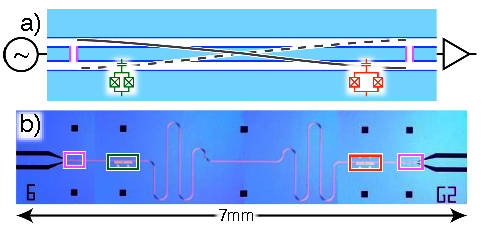
\includegraphics[width=\textwidth]{images/coupled_transmon}\\
    \hfill\tiny{Majer \emph{et al.} Nature 449, 443 (2007)}\hspace{2mm}~\\
  \end{textblock}
  \begin{textblock}{6}(9,2.25)
    \begin{equation*}
      \Op{H} = \Op{H}_0 + \epsilon(t) \Op{H}_1
    \end{equation*}
  \end{textblock}
  \begin{textblock}{5}(9.5,3.2)
    \begin{tikzpicture}
      \draw[->, line width = 1pt] (0, 0) -- +(0, 12pt);
      \node[below] (0,0) {microwave field in transmission line};
    \end{tikzpicture}
  \end{textblock}
  \begin{textblock}{4}(3,5.5)
    \includegraphics<2->[height=3cm]{images/YaoCircuit_cutout}
  \end{textblock}
  \begin{textblock}{10}(6,6.0)
    \onslide<2->{%
      \begin{equation*}
        \left.\begin{aligned}
        \ket{00} & \rightarrow \text{CR}_2 \ket{00} \\
        \ket{01} & \rightarrow \text{CR}_2 \ket{01} \\
        \ket{10} & \rightarrow \text{CR}_2 \ket{10} \\
        \ket{11} & \rightarrow \text{CR}_2 \ket{11}
        \end{aligned} \quad \right\} \quad \begin{aligned}
          & \text{with the same}~\epsilon(t); \\
          & \text{acting on logical subspace}
        \end{aligned}
      \end{equation*}
    }
  \end{textblock}
  \note<1>{%

    So, for example, if you have superconducting qubits you'd have something like this Transmon circuit,

    where you have two transmons with a shared transmission line, and the control you have is the field that you put into the transmission line.
  }
  \note<2>{%
    And now we're going to try to find a field so that every logical basis state for a two-qubit system evolves so that it implements this controlled rotation.

    \dots

    But there's other control problems besides implementing gates.
  }
\end{frame}


\begin{frame}{Controlling photo-chemical reactions}
 \begin{textblock}{7.5}(0.5,1.5)
   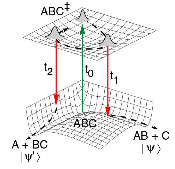
\includegraphics[width=0.95\textwidth]{images/tannor_rice_scheme}
 \end{textblock}
 \begin{textblock}{7.5}(8.0,1.25)
   \begin{itemize}
     \item Kosloff, Rice, et. al. \textit{Wavepacket dancing: Achieving chemical selectivity by shaping light pulses}. Chem. Phys. 139, 201 (1989).
     \item Tannor, Jin. \textit{Design of femtosecond pulse sequences to control photochemical products}, in \textit{Mode Selective Chemistry} (Springer, 1991)
     \item Shi, Rabitz. \textit{Optimal control of bond selectivity in unimolecular reactions}. Comput. Phys. Commun. 63, 71 (1991)
     \item Judson, Rabitz. \textit{Teaching lasers to control molecules}. Phys. Rev. Lett. 68, 1500 (1992).
   \end{itemize}
 \end{textblock}
\end{frame}


\begin{frame}{Tractor atom interferometry}
  \begin{textblock}{8.5}(0.75,1.5)
    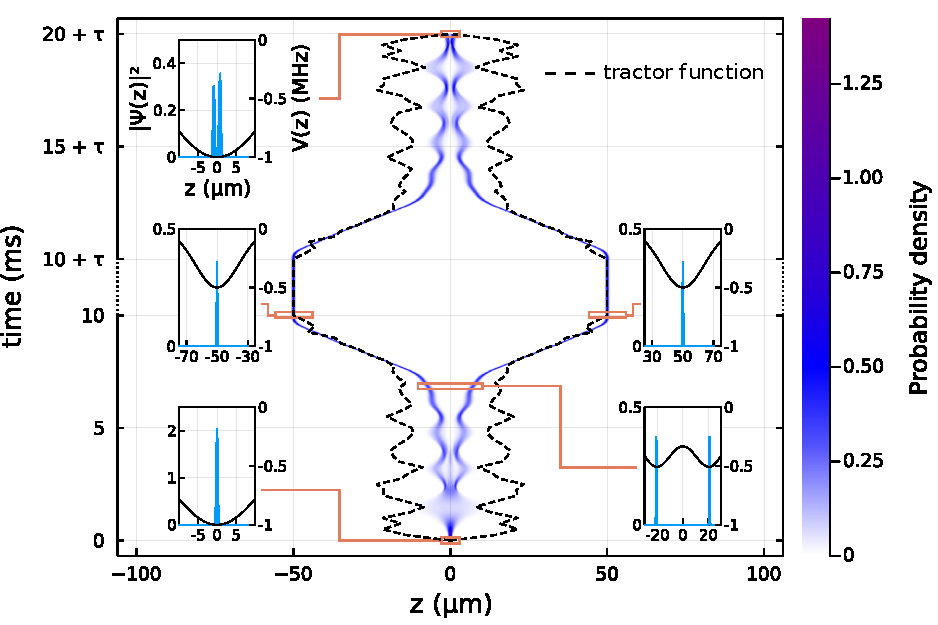
\includegraphics[width=\textwidth]{images/RaithelQST2022_Fig4}\\
    \footnotesize{Raithel \emph{et al.} Quantum Sci. Technol. 8, 014001 (2022)}
  \end{textblock}
  \begin{textblock}{6}(9.75,3.5)
    {\color{DarkRed}
      Find non-adiabatic tractor potential\\
      closing interferometric path
    }
  \end{textblock}
  \note<1>{%
    Or, something that's closer to what I'm doing these days,

    you could have some trapped atoms where you split them into two trapping potentials and then you move the potentials along two different pathways to implement an interferometer.

    And then you have to find exactly the right trajectory to combined the wavepackets again at the end.
  }
\end{frame}


\begin{frame}{Outline}
  \begin{itemize}
    \item Formulating the control problem
      \begin{itemize}
        \item Quantum gates with coupled transmon qubits
        \item Unconstrained control problems
      \end{itemize}
    \pause
    \item Gradient-ascent (GRAPE)
      \begin{itemize}
        \item Simulating time dynamics
        \item Evaluating gradients
        \item Semi-automatic differentiation: evaluate arbitrary functionals
        \item Example: Maximizing gate entanglement
      \end{itemize}
    \pause
    \item Krotov's method
    \pause
    \item QuantumControl.jl: efficiently implementing quantum control
    \pause
    \item Parametrized and constrained control problems
  \end{itemize}
\end{frame}


\begin{frame}{Quantum gates with coupled transmon qubits}
  \begin{textblock}{15.0}(0.5,1.75)
    \begin{center}
      \only<1>{%
        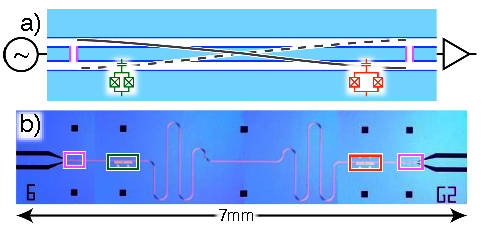
\includegraphics[width=0.7\textwidth]{images/coupled_transmon}\\
        \hfill{\small Majer \emph{et al.} Nature 449, 443 (2007)}\hspace{2mm}~\\
      }
      \only<2>{%
        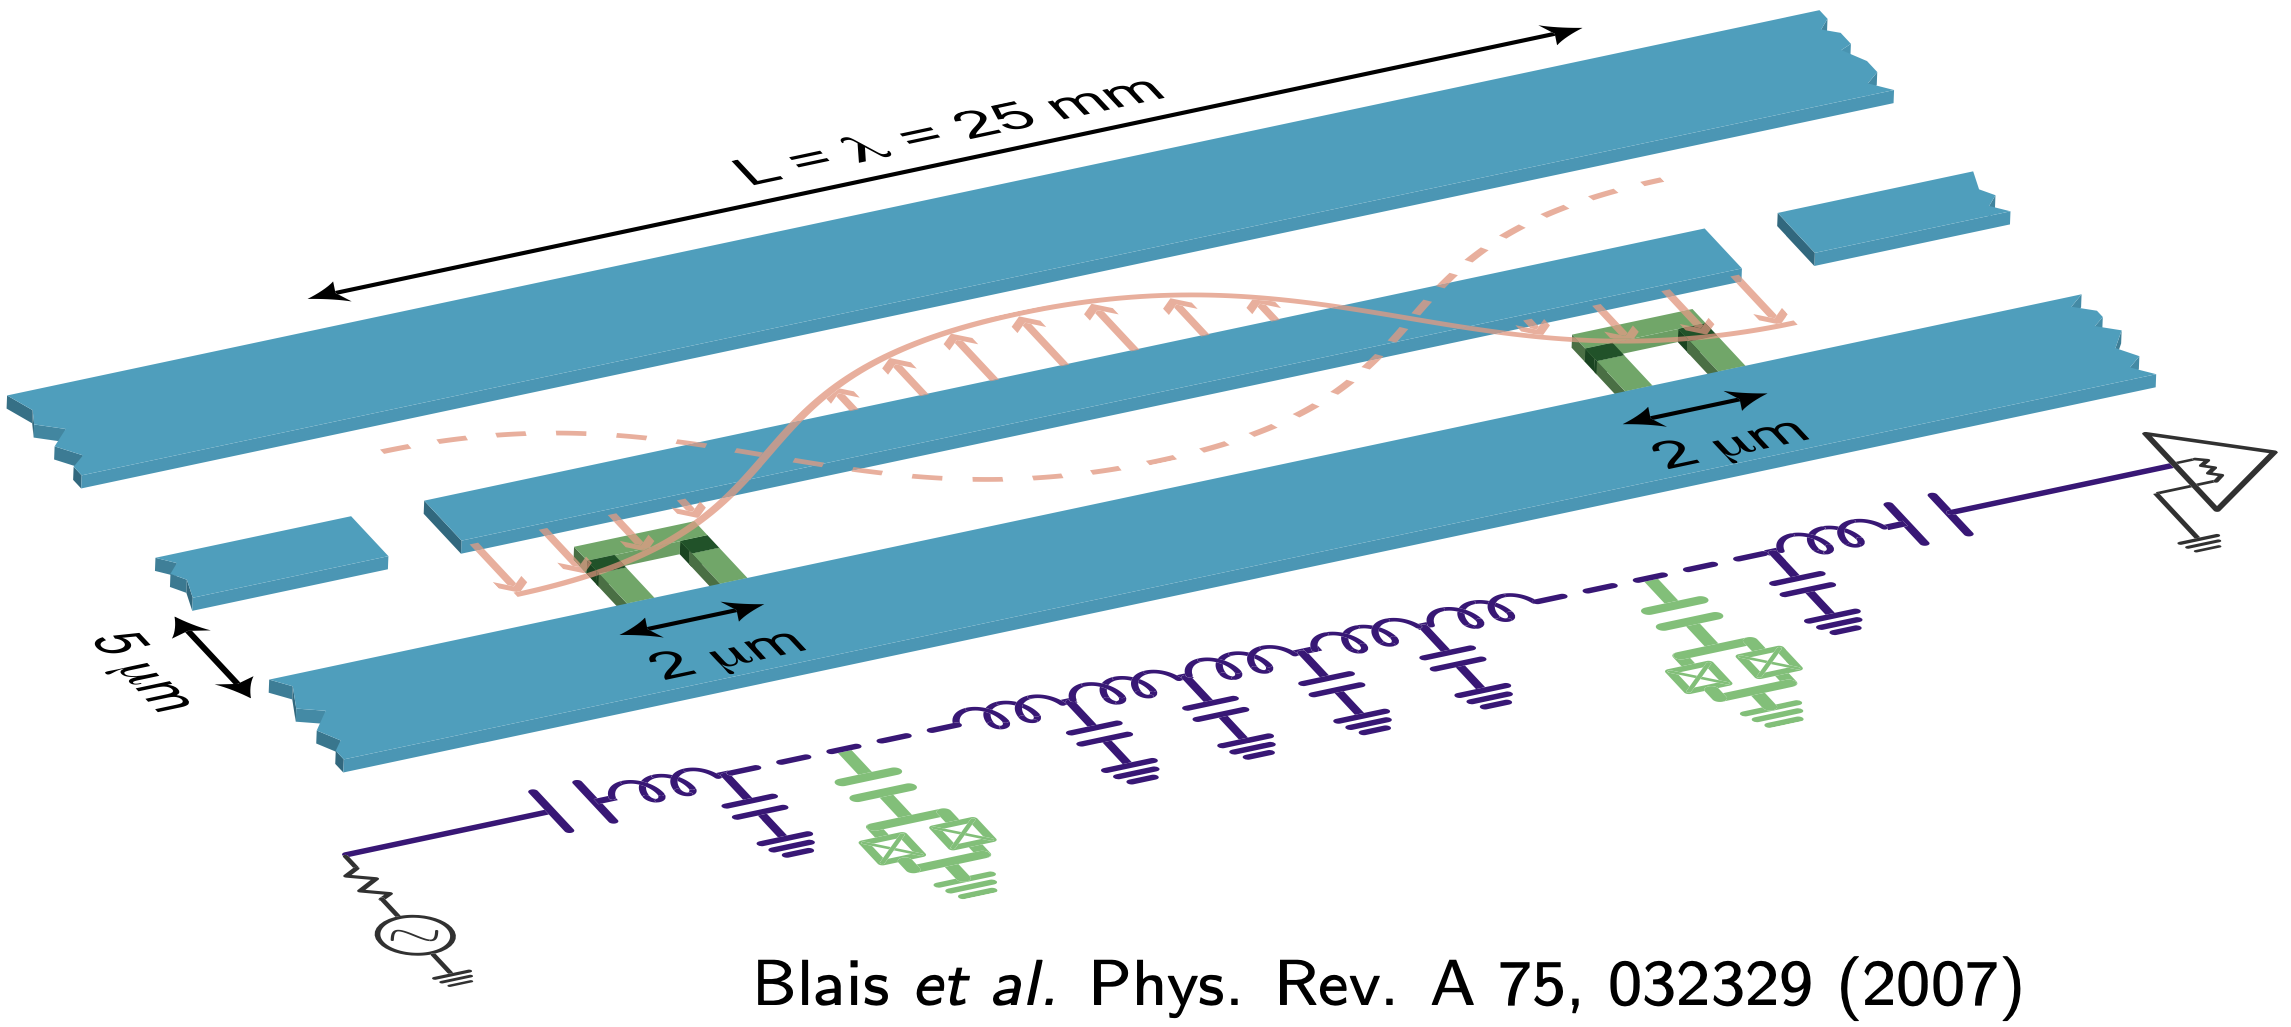
\includegraphics[width=0.8\textwidth]{images/coupled_transmon_dispersive}
      }
    \end{center}
  \end{textblock}
\end{frame}


\begin{frame}
  \begin{textblock}{15.0}(0.5,0.3)
    \begin{center}
      \includegraphics<1>[height=8.0cm]{images/blackboard_01}
      \includegraphics<2>[height=8.0cm]{images/blackboard_02}
      \includegraphics<3>[height=8.0cm]{images/blackboard_03}
      \includegraphics<4>[height=8.0cm]{images/blackboard_04}
    \end{center}
  \end{textblock}
\end{frame}


\begin{frame}{Time Discretization}
  \begin{textblock}{6.5}(0.5,1.00)
    \includegraphics<1>{images/pulse_examples_simple}
    \includegraphics<2>{images/pulse_examples_continuous}
    \includegraphics<3>{images/pulse_examples_discrete}
    \includegraphics<4->{images/pulse_examples_pwc}
  \end{textblock}
  \begin{textblock}{7}(8.25,1.00)
    \begingroup
      \addtolength{\jot}{1em}  % increase space between rows
      \begin{align*}
        i \hbar \frac{\partial}{\partial t} \ket{\Psi(t)} &= \Op{H}(\{\epsilon_l(t)\}) \ket{\Psi(t)}\\
        i \hbar \frac{\partial}{\partial t} \hat\rho(t) &= \Liouvillian(\{\epsilon_l(t)\})[\hat\rho(t)]
      \end{align*}
    \endgroup
  \end{textblock}
  \begin{textblock}{14}(1.0,4.45)
    \onslide<5->{%
      \begin{center}
        Piecewise constant: {$\Op{H}_n = \Op{H}(\{\epsilon_{nl}\})$ with $\epsilon_{nl} = \epsilon_l(t=t_n)$} for $n$'th time slice
      \end{center}
    }
  \end{textblock}
  \begin{textblock}{14}(1.0,5.9)
    \onslide<6->{%
      \begin{equation*}
        J(\{\only<6>{\epsilon_l(t)}\only<7->{{\color{DarkRed}\epsilon_{nl}}}\}) = J_T(\{\ket{\Psi_k(T)}\}) + \int_{0}^T \dots dt
      \end{equation*}
      \vspace{-2pt}
      \begin{center}
        \onslide<8->{%
          Gradient {\color{DarkRed}$\nabla J \equiv \frac{\partial{J}}{{\partial \epsilon_{nl}}}$}
          \onslide<9->{$\quad \Rightarrow \quad$ LBFGS}
        }
      \end{center}
    }
  \end{textblock}
\end{frame}


\begin{frame}
  \begin{textblock}{15}(0.5,2.50)
    \begin{center}
      \Large
      Gradient Ascent Pulse Engineering (GRAPE)
    \end{center}
    \vspace{3mm}
    \begin{center}
      How to calculate $\nabla J$ for PWC controls
    \end{center}
  \end{textblock}
  \begin{textblock}{15}(0.5,6.50)
    Khaneja, Reiss, Kehlet, Schulte-Herbrüggen, Glaser.
    \textit{Optimal control of coupled spin dynamics: Design of NMR pulse sequences by gradient ascent algorithms}. \\
    J. Magnet. Res. 172, 296 (2005)
  \end{textblock}
\end{frame}


\begin{frame}
  \begin{textblock}{15.0}(0.5,0.3)
    \begin{center}
      \includegraphics<1>[height=8.0cm]{images/blackboard_06}
    \end{center}
  \end{textblock}
\end{frame}


\begin{frame}{Aside: Wirtinger derivatives --- derivatives w.r.t. complex numbers}
  %\begin{textblock}{3.0}(0.5,1.0)
    \begin{equation*}
      J_T (\{\tau_k\}) = J_T(\{\Re[\tau_k], \Im[\tau_k]\}); \qquad J_T \in \Reals, \quad \tau_k \in \Complex
    \end{equation*}
    \pause
    \begin{equation*}
      \frac{\partial J_T (\{\tau_k\})}{\partial \epsilon_{nl}} =
      \sum_k \left(
        \frac{\partial J_T}{\partial \Re[\tau_k]}
        \frac{\partial \Re[\tau_k]}{\partial \epsilon_{nl}}
        + \frac{\partial J_T}{\partial \Im[\tau_k]}
        \frac{\partial \Im[\tau_k]}{\partial \epsilon_{nl}}
      \right);
      \qquad \epsilon_{nl} \in \Reals
    \end{equation*}
    \pause
    {
      \color{DarkRed}
      \begin{align*}
        \text{Define} \quad \frac{\partial J_T (\{\tau_k\})}{\partial \tau_k}
        & \equiv \frac{1}{2} \left(
          \frac{\partial J_T}{\partial \Re[\tau_k]}
          - i \frac{\partial J_T}{\partial \Im[\tau_k]}
        \right) \\
        \frac{\partial J_T (\{\tau_k\})}{\partial \tau_k^*}
        & \equiv \frac{1}{2} \left(
          \frac{\partial J_T}{\partial \Re[\tau_k]}
          + i \frac{\partial J_T}{\partial \Im[\tau_k]}
        \right)
        = \left(\frac{\partial J_T}{\partial \tau_k}\right)^*
      \end{align*}
    }
    \vspace{1mm}
    \pause
    \begin{equation*}
       \frac{\partial J_T (\{\tau_k\})}{\partial \epsilon_{nl}}
       =
       \sum_k \left(
         \frac{\partial J_T}{\partial \tau_k}
         \frac{\partial \tau_k}{\partial \epsilon_{nl}}
         + \frac{\partial J_T}{\partial \tau_k^*}
         \frac{\partial \tau_k^*}{\partial \epsilon_{nl}}
       \right)
      =
       2 \Re \left[
        \sum_k
        \frac{\partial J_T}{\partial \tau_k} \frac{\partial \tau_k}{\partial \epsilon_{nl}}
       \right]
    \end{equation*}
  %\end{textblock}
\end{frame}


\begin{frame}
  \begin{textblock}{15.0}(0.5,0.3)
    \begin{center}
      \includegraphics<1>[height=8.0cm]{images/blackboard_08}
    \end{center}
  \end{textblock}
\end{frame}

\begin{frame}{Piecewise-constant time propagation}
  \begin{textblock}{6.5}(0.5,1.00)
    \includegraphics<1->{images/pulse_examples_pwc}
  \end{textblock}
  \begin{textblock}{7}(8.25,1.00)
    \begingroup
      \addtolength{\jot}{1em}  % increase space between rows
      \begin{align*}
        i \hbar \frac{\partial}{\partial t} \ket{\Psi(t)} &= \Op{H}(\{\epsilon_l(t)\}) \ket{\Psi(t)}\\
        i \hbar \frac{\partial}{\partial t} \hat\rho(t) &= \Liouvillian(\{\epsilon_l(t)\})[\hat\rho(t)]
      \end{align*}
    \endgroup
  \end{textblock}
  \begin{textblock}{14}(1.0,4.45)
    \onslide<2->{%
      \begin{center}
        PWC propagator: {\color{DarkRed}$\Op{U}_n = \exp[-\frac{i}{\hbar} \Op{H}_n dt]$} for $n$'th time slice
      \end{center}
    }
  \end{textblock}
  \begin{textblock}{14}(1.0,5.95)
    \onslide<3->{%
      $\Rightarrow$ evaluate $\Op{U}_n \ket{\Psi}$ (or $\mathcal{U}_n[\hat\rho]$) as a polynomial expansion
      \vspace{5mm}
      \onslide<4->{
        \begin{itemize}
          \item Hermitian Hamiltonian $\rightarrow$ Chebychev polynomials
          \item Non-Hermitian Hamiltonian or Liouvillian $\rightarrow$ Newton polynomials
        \end{itemize}
      }
    }
  \end{textblock}
\end{frame}

\begin{frame}{Chebychev Propagation}
  \begin{textblock}{14}(1.0, 1.25)
    \onslide<1->{%
      \subhead{Chebychev Polynomials}
        \onslide<1->{%
          \begin{equation*}
            P_0(x)  = 1;\quad
            P_1(x)  = x;\quad
            P_n(x)  = 2x P_n(x) - P_{n-1}(x)
          \end{equation*}
          $P_n(x) \quad \text{ are defined for } \quad x \in [-1, 1]$
        }
    }
  \end{textblock}
  \begin{textblock}{14}(1.0, 4.35)
    \onslide<2->{%
      \begin{equation*}
        \Ket{\Psi(t+dt)}
        = e^{-\ii \Op{H} \,dt} \Ket{\Psi(t)}
        = \sum_{n} a_n \underbrace{P_n(-\ii \Op{H}_{\text{norm}}) \Ket{\Psi(t)}}_{%
                                              \equiv \Ket{\Phi_n}}\,,
      \end{equation*}
    }
  \end{textblock}
  \begin{textblock}{14}(1.0, 5.65)
    \onslide<3->{%
      \begin{equation*}
        \Op{H}_{\norm} = 2 \frac{\Op{H} - E_{\min}\,\identity}{\Delta} - \identity\,,\qquad
        a_n = (2-\delta_{n0})
              e^{-\frac{\ii}{\hbar} \left( \frac{\Delta}{2} + E_{\min}\right)\,dt}
              J_k(\alpha)\,,
      \end{equation*}
      \begin{equation*}
        \ket{\Phi_0(x)}  = \ket{\Psi(t)};\quad
        \ket{\Phi_1(x)}  = -\ii \Op{H}_{\norm} \Ket{\Phi_0};\quad
        \ket{\Phi_n(x)}  = -2\ii \Op{H}_{\norm} \Ket{\Phi_{n-1}} + \Ket{\Phi_{n-2}}
      \end{equation*}
    }
  \end{textblock}
\end{frame}

\begin{frame}{Chebychev Propagation – Pseudocode}
  \begin{textblock}{15}(0.5, 1.5)
    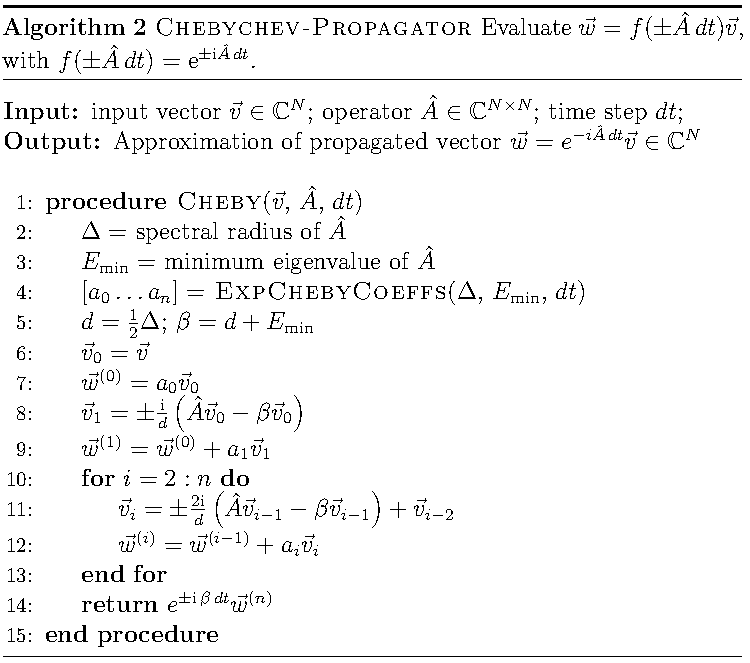
\includegraphics[width=0.49\textwidth]{images/chebyalg1}
    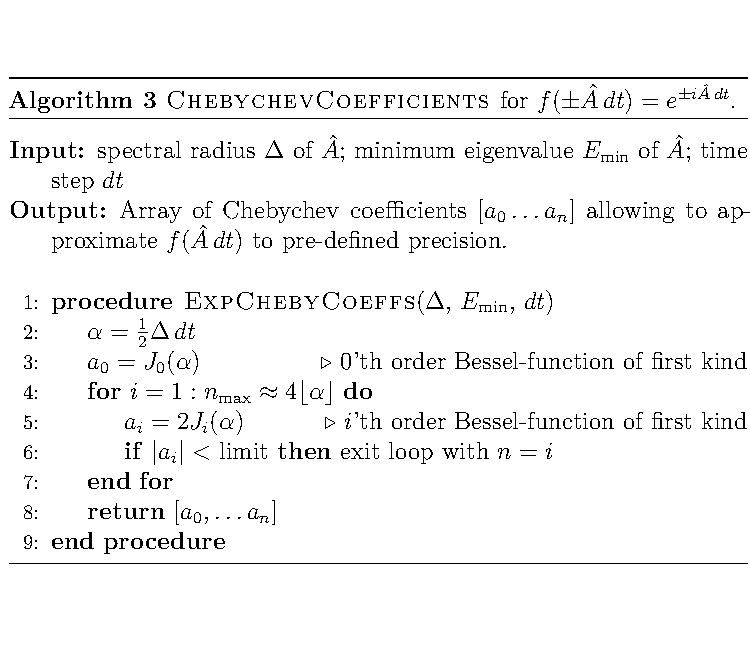
\includegraphics[width=0.49\textwidth]{images/chebyalg2}
    \par
    {\footnotesize
    \vspace{-7mm}
    \hfill
    Goerz, PhD Thesis, Appendix F\\
    \hfill
    \url{https://michaelgoerz.net}
    }
  \end{textblock}
\end{frame}

\begin{frame}
  \begin{textblock}{15.5}(0.25,0.2)
    {\footnotesize
      \url{https://github.com/JuliaQuantumControl/QuantumPropagators.jl}
    }
  \end{textblock}
  \begin{textblock}{15.5}(0.25,0.5)
    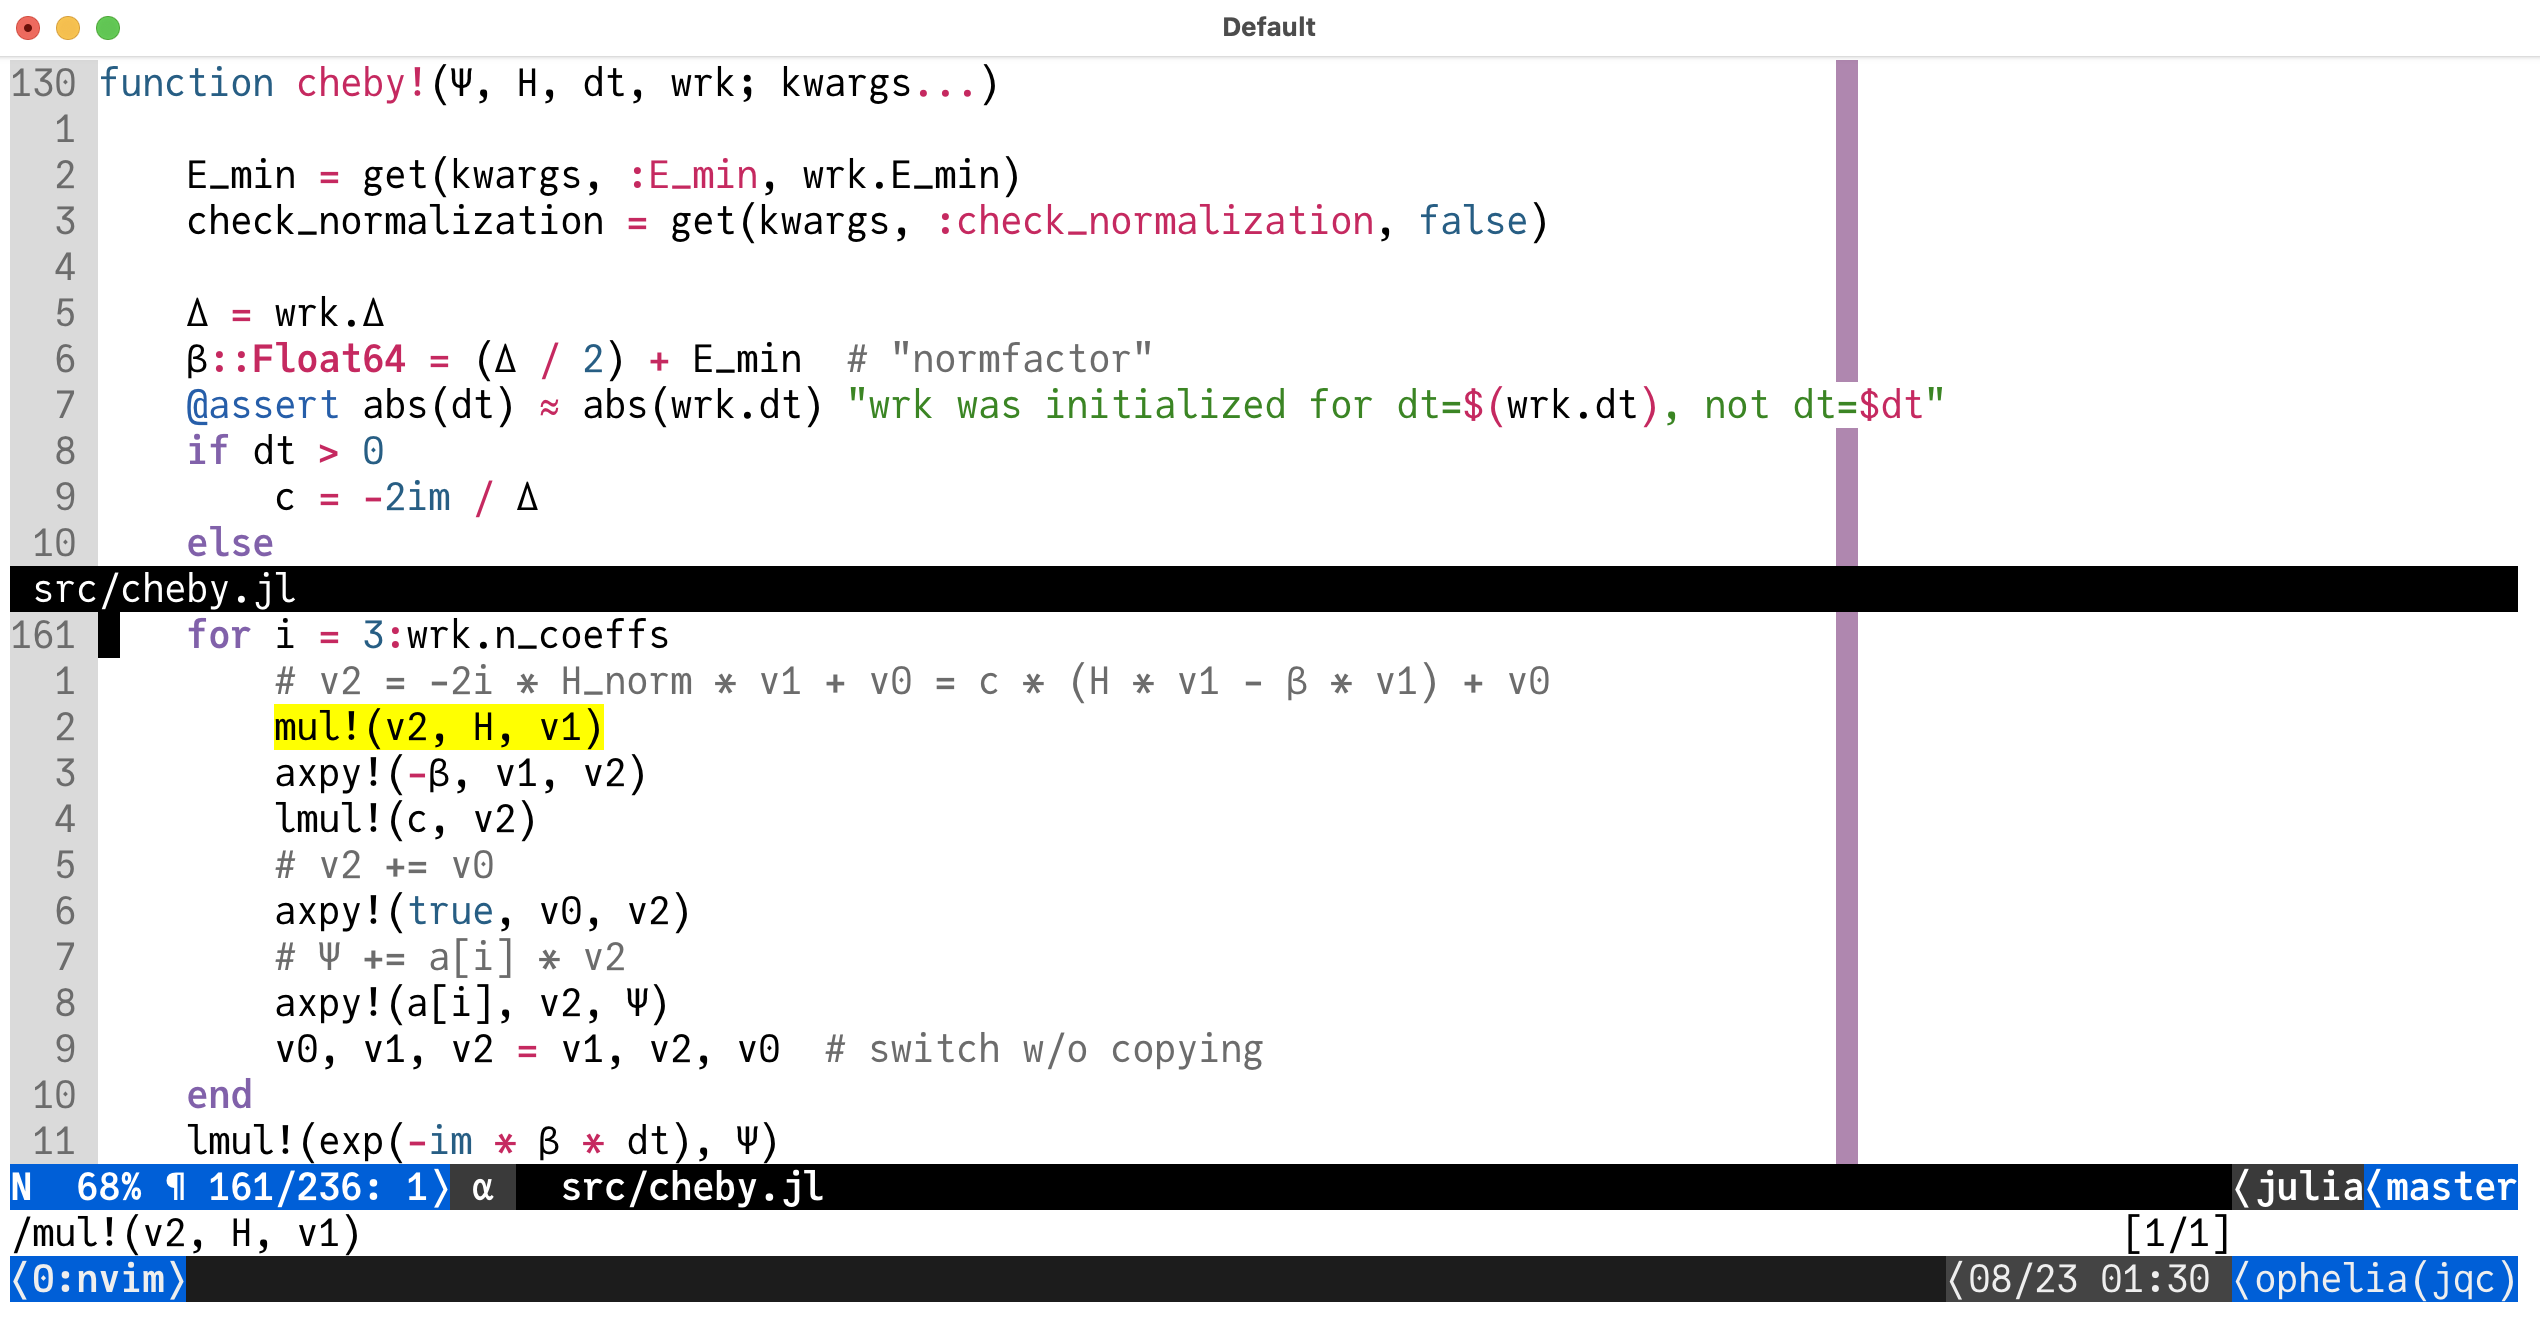
\includegraphics[width=\textwidth]{images/cheby_implementation}
  \end{textblock}
\end{frame}


\begin{frame}{Gradient of Time Evolution Operator}
    \begin{equation*}%
      \begin{pmatrix}
        \frac{\partial \Op{U}^{\dagger}_n}{\partial \epsilon_{n1}} \ket{\chi_k(t_{n})} \\
          \vdots\\
          \frac{\partial \Op{U}^{\dagger}_n}{\partial \epsilon_{nL}} \ket{\chi_k(t_{n})} \\
          \Op{U}^{\dagger}_n \ket{\chi_k(t_{n})}
        \end{pmatrix}
      = \exp \left[-\ii \begin{pmatrix}
        \Op{H}^\dagger_n & 0 & \dots & 0 &\Op{H}_n^{(1)\dagger} \\
        0 & \Op{H}^\dagger_n & \dots & 0 & \Op{H}_n^{(2)\dagger} \\
        \vdots & & \ddots & & \vdots \\
        0 & 0 & \dots & \Op{H}^\dagger_n & \Op{H}_n^{(L)\dagger} \\
        0 & 0 & \dots & 0 & \Op{H}^\dagger_n\,,
      \end{pmatrix} dt_n\right]
      \begin{pmatrix} 0 \\ \vdots \\ 0 \\ \ket{\chi_k(t_n)} \end{pmatrix}
    \end{equation*}
    \vspace{5mm}
    \begin{equation*}
      \Op{U}_n = \exp[-\ii \Op{H}_n dt_n]\,;
      \qquad
      \Op{H}_n^{(l)} = \frac{\partial \Op{H}_n}{\partial \epsilon_l(t)}
    \end{equation*}
    \par
    \vspace{5mm}
    \hfill \footnotesize{--- Goodwin, Kuprov, J. Chem. Phys. 143, 084113 (2015)}\\
    \vspace{3mm}
    \hfill \footnotesize{\url{https://github.com/JuliaQuantumControl/QuantumGradientGenerators.jl}}
\end{frame}



\begin{frame}{Optimizing for a Maximally Entangling Gate}
  \begin{textblock}{5.25}(10.5,2.50)
    \includegraphics<2->[width=\textwidth]{images/weylchamber}
  \end{textblock}
  \begin{textblock}{14}(0.5, 1.60)
    \onslide<2->{%
      \subhead{Cartan decomposition}
      \begin{equation*}
        \Op{U} = \Op{k}_1 \exp\left[ \frac{\ii}{2} \left(
                      {\color{Red}c_1} \SigmaX\SigmaX
                    + {\color{Red}c_2} \SigmaY\SigmaY
                    + {\color{Red}c_3} \SigmaZ\SigmaZ
                  \right) \right] \Op{k}_2
      \end{equation*}
      $\Op{k}_{1,2}$: Single qubit gates; \hspace{24pt}
      $c_{1,2,3}$: Weyl chamber coordinates
    }
  \end{textblock}
  \begin{textblock}{9.5}(0.5,4.85)
    \only<3->{%
      \subhead{Gate concurrence of two-qubit gate $\Op{U}$}
      \vspace{3mm}
      \begin{enumerate}
        \item
          $
            c_1, c_2, c_3 \propto
            \text{eigvals}\left( \Op{U} \TildeOp{U} \right)\,;\quad
            \TildeOp{U} = (\Op{\sigma}_y \otimes \Op{\sigma}_y) \,\Op{U}\, (\Op{\sigma}_y \otimes \Op{\sigma}_y)
          $
        \item
          $
            C(\Op{U})
              = \max \Abs{\sin(c_{1,2,3} \pm c_{3,1,2})}
          $
      \end{enumerate}
      \hfill {\footnotesize Childs \textit{et al.} Phys. Rev. A 68, 052311 (2003)}\\
      \only<4>{\vspace{6pt}\hspace{10mm}{\color{Red} \bf Not analytic!}}
    }
  \end{textblock}
\end{frame}


\begin{frame}{Automatic differentiation (AD)}
  \begin{textblock}{14}(1.0,1.0)
    \only<1>{%
      \vspace{12mm}
      \begin{itemize}
        \item Build computational graph for time propagation
        \item Elementary operations have known derivatives
        \item Let computer apply chain rule at each node in graph
        \item Backward pass to accumulate gradient
      \end{itemize}
      \vspace{16mm}
      \begin{itemize}
        \footnotesize
      \item[---] Leung \textit{et al.} Phys. Rev. A 95, 042318 (2017)
      \item[---] Abdelhafez \textit{et al.}, Phys. Rev. A 99, 052327 (2019)
      \item[---] Schäfer, \textit{et al.} Mach. Learn.: Sci. Technol. 1, 035009 (2020)
      \item[---] Abdelhafez \textit{et al.} Phys. Rev. A 101, 022321 (2020)
      \end{itemize}
    }
    \only<2>{%
      \begin{center}
        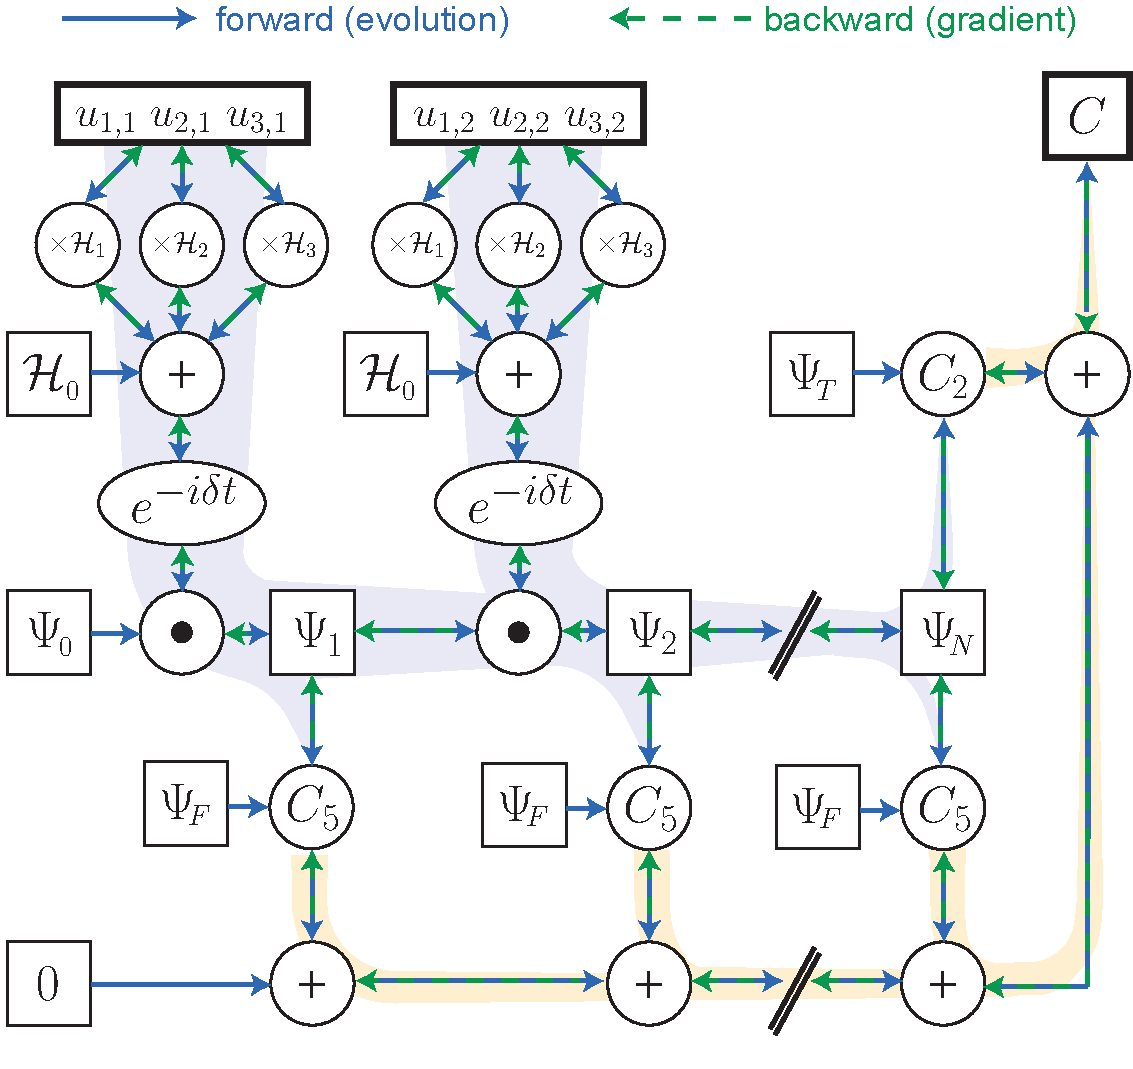
\includegraphics[width=0.5\textwidth]{images/nn_graph}\\
        {\footnotesize Fig. 2 in Leung \emph{et al.} Phys. Rev. A 95, 042318 (2017)}
      \end{center}
    }
  \end{textblock}
\end{frame}

\begin{frame}
  \begin{textblock}{15.0}(0.5,0.3)
    \begin{center}
      \includegraphics<1>[height=8.0cm]{images/blackboard_10}
    \end{center}
  \end{textblock}
\end{frame}

\begin{frame}{Generalized GRAPE scheme}
  \begin{textblock}{15}(0.5,1.0)
    \begin{center}
      %\documentclass[a0,landscape]{a0poster}
%\pdfoutput=1
%\usepackage{xcolor}
%\usepackage{amsmath}
%\usepackage{amsfonts}
%\usepackage{braket}
%\newcommand{\Op}[1]{\ensuremath{\mathsf{\hat{#1}}}}
%\newcommand{\tgt}{\text{tgt}}
%\newcommand{\ii}{\mathrm{i}}
%\renewcommand{\Re}{\mathrm{Re}}
%\renewcommand{\Im}{\mathrm{Im}}
%\newcommand{\Liouville}[0]{\mathcal{L}}
%\newcommand{\identity}[0]{\mathbf{1}}
\def\guesslbl{(0)}
\def\iterlbl{(1)}
%\DeclareMathSymbol{\shortminus}{\mathbin}{AMSa}{"39}
%\renewcommand{\familydefault}{\sfdefault}
%\definecolor{DarkBlue}{rgb}{0.1,0.1,0.5}
%\definecolor{DarkRed}{rgb}{0.75,0.,0.}
%
%\usepackage{tikz}
%
%\usepackage[psfixbb,graphics,tightpage,active]{preview}
%\PreviewEnvironment{tikzpicture}
%
%\begin{document}
%%%%%%%%%%%%%%%%%%%%%%%%%%%%%%%%%%%%%%%%%%%%%%%%%%%%%%%%%%%%%%%%%%%%%%%%%%%%%%%%
\begin{tikzpicture}[
  x=0.85cm,
  y=0.6cm,
  very thick,
]
\tikzstyle{every node}+=[font= \footnotesize ]
\tikzstyle{fwproparrow}=[transform canvas={yshift=-10pt}, bend right=50]
\tikzstyle{bwproparrow}=[transform canvas={yshift=10pt}, bend left=50]
\tikzstyle{gradlabel}=[below=3pt,color=DarkBlue]
\tikzstyle{updatelabel}=[above=3pt,color=DarkBlue]

\begin{scope}

  %\node[anchor=west] at (1.7, 11.5) {(a) GRAPE};

  \onslide<2->{
  %%% propagation boxes
  % lower
  \draw[color=gray!20, fill=gray!20,rounded corners=5] (2,0.1) rectangle +(14,4.55);
  \node[align=center] at (9, 0.5){\raisebox{.5pt}{\textcircled{\raisebox{-.9pt} {1}}} forward-prop and storage with guess};

  %%% forward propagation

  \node (psifw1) at (3,4.0) {%
    \begin{tikzpicture}[very thick]
      \draw (-0.3,0)--(0.5,-0.25)--(1.3,0);
      \node[color=DarkRed] at (0.5,0.55) {$\phi_k$};
    \end{tikzpicture}
  };

  \node (psifw2) at (6,4.0) {%
    \begin{tikzpicture}[very thick]
      \draw (-0.3,0)--(0.5,-0.25)--(1.3,0);
      \node[color=DarkRed] at (0.5,0.55) {$\Psi_k(t_1)$};
    \end{tikzpicture}
  };
  \draw[->] (psifw1) edge[fwproparrow] node[below]{$\epsilon^{\guesslbl}_{l,1}$} (psifw2);

  \node (psifw3) at (9,4.0) {%
    \begin{tikzpicture}[very thick]
      \draw[color=gray!20] (-0.3,0)--(0.5,-0.25)--(1.3,0);
      \node[color=gray!20] at (0.5,0.55) {$\Psi_k(t)$};
      \node at (0.5,0.35) {\dots};
    \end{tikzpicture}
  };
  \draw[->] (psifw2) edge[fwproparrow] node[below]{$\epsilon^{\guesslbl}_{l,2}$} (psifw3);

  \node (psifw4) at (12,4.0) {%
    \begin{tikzpicture}[very thick]
      \draw (-0.3,0)--(0.5,-0.25)--(1.3,0);
      \node[color=DarkRed] at (0.5,0.55) {$\Psi_k(t_{N_T-1})$};
    \end{tikzpicture}
  };
  \draw[->] (psifw3) edge[fwproparrow] node[below]{$\epsilon^{\guesslbl}_{l,N_T-1}$} (psifw4);

  \node (psifw5) at (15,4.0) {%
    \begin{tikzpicture}[very thick]
      \node[color=DarkRed] at (0.5,0.55) {$\Psi_k(T)$};
    \end{tikzpicture}
  };
  \draw[->] (psifw4)  edge[fwproparrow] node[below]{$\epsilon^{\guesslbl}_{l, N_T}$} (psifw5);
  }

  %%% backward propagation

  \onslide<3->{
  % upper
  \draw[color=gray!20, fill=gray!20,rounded corners=5] (2,6.35) rectangle +(14,4.55);
    \node[align=center] at (9, 10.5){\raisebox{.5pt}{\textcircled{\raisebox{-.9pt} {2}}} backward-prop of extended state/gradient};

  \node (chi1) at (3,7.0) {%
    \begin{tikzpicture}[very thick]
      \draw (-0.3,0)--(0.5,0.25)--(1.3,0);
      \node at (0.5,-0.55) {$\tilde\chi_k(0)$};
    \end{tikzpicture}
  };

  \node (chi2) at (6,7.0) {%
    \begin{tikzpicture}[very thick]
      \draw (-0.3,0)--(0.5,0.25)--(1.3,0);
      \node at (0.5,-0.55) {$\tilde\chi_k(t_1)$};
    \end{tikzpicture}
  };
  \draw[<-] (chi1) edge[bwproparrow] node[above]{$\epsilon^{\guesslbl}_{l,1}$} node(gradn1)[gradlabel]{$\nabla\!\tau^{(k)}_{l,1}$} (chi2);

  \node (chi3) at (9,7.0) {%
    \begin{tikzpicture}[very thick]
      \draw[color=gray!20] (-0.3,0)--(0.5,0.25)--(1.3,0);
      \node[color=gray!20] at (0.5,-0.25) {$\tilde\chi_k(t)$};
      \node at (0.5,-0.55) {\dots};
    \end{tikzpicture}
  };
  \draw[<-] (chi2)  edge[bwproparrow] node[above]{$\epsilon^{\guesslbl}_{l,2}$} node(gradn2)[gradlabel]{$\nabla\!\tau^{(k)}_{l,2}$} (chi3);

  \node (chi4) at (12,7.0) {%
    \begin{tikzpicture}[very thick]
      \draw (-0.3,0)--(0.5,0.25)--(1.3,0);
      \node at (0.5,-0.55) {$\tilde\chi_k(t_{N_T-1})$};
    \end{tikzpicture}
  };
  \draw[<-] (chi3) edge[bwproparrow] node[above]{$\epsilon^{\guesslbl}_{l,N_T-1}$} node(gradn3)[gradlabel]{$\nabla\!\tau^{(k)}_{l,N_T-1}$}(chi4);

  \node (chi5) at (15,7.0) {%
    \begin{tikzpicture}[very thick]
      \draw[color=gray!20] (-0.3,0)--(0.5,0.25)--(1.3,0);
      \node[] at (0.5,-0.55) {$\tilde\chi_k(T)$};
    \end{tikzpicture}
  };
  \draw[<-] (chi4) edge[bwproparrow] node[above]{$\epsilon^{\guesslbl}_{l, N_T}$} node(gradn4)[gradlabel]{$\nabla\!\tau^{(k)}_{l, N_{T}}$} (chi5);

  %%% mu
  \node (mu1) at (3,5.5) {%
    \begin{tikzpicture}[very thick]
      \draw (-0.8,0.0)--(0.8,0.0);
    \end{tikzpicture}
  };
  \draw[->,color=DarkBlue] (mu1) -| (gradn1);

  \node (mu2) at (6,5.5) {%
    \begin{tikzpicture}[very thick]
      \draw (-0.8,0.0)--(0.8,0.0);
    \end{tikzpicture}
  };
  \draw[->,color=DarkBlue] (mu2) -| (gradn2);

  \node (mu3) at (9,5.5) {%
    \begin{tikzpicture}[very thick]
      \draw[opacity=0] (-0.8,0.6)--(0.8,0.6);
      \node at (0,0) {\dots};
      \draw[opacity=0] (-0.8,-0.6)--(0.8,-0.6);
    \end{tikzpicture}
  };
  \draw[->,color=DarkBlue] (mu3) -| (gradn3);

  \node (mu4) at (12,5.5) {%
    \begin{tikzpicture}[very thick]
      \draw (-0.8,0.0)--(0.8,0.0);
    \end{tikzpicture}
  };
  \draw[->,color=DarkBlue] (mu4) -| (gradn4);
  }


\end{scope}


\end{tikzpicture}

%%%%%%%%%%%%%%%%%%%%%%%%%%%%%%%%%%%%%%%%%%%%%%%%%%%%%%%%%%%%%%%%%%%%%%%%%%%%%%%%
%
%\end{document}

    \end{center}
  \end{textblock}
  \begin{textblock}{3}(11.5, 1.4)
    \begin{tikzpicture}
      \draw<4-> (0,0) node[line width = 3pt, draw=black, inner sep = 6pt, fill=gray!20,rounded corners=10] {
        $\tau^{(k)} = \Braket{\chi_k(T)|\Psi_k(T)}$
      };
    \end{tikzpicture}
  \end{textblock}
  \begin{textblock}{3}(0.3, 1.4)
    \begin{tikzpicture}
      \draw<5-> (0,0) node[line width = 3pt, draw=black, inner sep = 6pt, fill=gray!20,rounded corners=10] {
        $\nabla J_T = 2 \Re \sum_k \nabla \tau^{(k)}$
      };
    \end{tikzpicture}
  \end{textblock}
  \begin{textblock}{15}(0.5,8.15)
    \hfill \footnotesize{--- Goerz \emph{et al.} Quantum 6, 871 (2022)}
  \end{textblock}
\end{frame}


\begin{frame}
  \begin{textblock}{15.5}(0.25,0.5)
    \includegraphics<1>[width=\textwidth]{images/example01} % still image
  \end{textblock}
  \begin{textblock}{12}(2.0,7.0)
    \begin{center}
      \begin{block}
        \large
        \url{https://github.com/JuliaQuantumControl/JuliaCon2023-Demo}
      \end{block}
    \end{center}
  \end{textblock}
\end{frame}


\begin{frame}
  \vspace{8mm}
  GRAPE: discretize first, then calculate gradient
  \par
  \vspace{8mm}
  \pause
  Alternative: variational calculus $\frac{\partial J}{\partial \epsilon(t)}$ --- \emph{then} discretize
  \pause
  \vspace{5mm}
  \begin{itemize}
    \item Adjoint method: add TDSE as constraint with Lagrage multiplier $\bra{\chi_k}$
      {\footnotesize
      \begin{itemize}
        \item[---] Shi, Rabitz, J. Chem. Phys. 92, 364 (1990)
        \item[---] Zhu, Botina, Rabitz, J. Chem. Phys. 108, 1953 (1998)
      \end{itemize}
      }
    \pause
      \vspace{5mm}
    \item Krotov's method: constructive approach
      {\footnotesize
      \begin{itemize}
        \item[---] Krotov, Feldman, Eng. Cybern. 21, 123 (1983)
        \item[---] Tannor, Kazakov, Orlov. In  \textit{Time-dependent quantum molecular dynamics} (1992)
        \item[---]  Reich, Ndong, Koch. J. Chem. Phys. Physics 136, 104103 (2012)
        \item[---]  Goerz \textit{et al.} SciPost Phys. 7, 080 (2019) [Python implementation]
      \end{itemize}
      }
  \end{itemize}
\end{frame}


\begin{frame}
  \begin{textblock}{15.0}(0.5,0.3)
    \begin{center}
      \includegraphics<1>[height=8.0cm]{images/blackboard_12}
    \end{center}
  \end{textblock}
\end{frame}

\begin{frame}{Krotov Numerical Scheme}
  \begin{textblock}{15}(0.5,1.0)
    \begin{center}
      %\documentclass[a0,landscape]{a0poster}
%\pdfoutput=1
%\usepackage{xcolor}
%\usepackage{amsmath}
%\usepackage{amsfonts}
%\usepackage{braket}
%\newcommand{\Op}[1]{\ensuremath{\mathsf{\hat{#1}}}}
%\newcommand{\tgt}{\text{tgt}}
%\newcommand{\ii}{\mathrm{i}}
%\renewcommand{\Re}{\mathrm{Re}}
%\renewcommand{\Im}{\mathrm{Im}}
%\newcommand{\Liouville}[0]{\mathcal{L}}
%\newcommand{\identity}[0]{\mathbf{1}}
\def\guesslbl{(0)}
\def\iterlbl{(1)}
%\DeclareMathSymbol{\shortminus}{\mathbin}{AMSa}{"39}
%\renewcommand{\familydefault}{\sfdefault}
%\definecolor{DarkBlue}{rgb}{0.1,0.1,0.5}
%\definecolor{DarkRed}{rgb}{0.75,0.,0.}
%
%\usepackage{tikz}
%
%\usepackage[psfixbb,graphics,tightpage,active]{preview}
%\PreviewEnvironment{tikzpicture}
%
%\begin{document}
%%%%%%%%%%%%%%%%%%%%%%%%%%%%%%%%%%%%%%%%%%%%%%%%%%%%%%%%%%%%%%%%%%%%%%%%%%%%%%%%
\begin{tikzpicture}[
  x=0.85cm,
  y=0.6cm,
  very thick,
]
\tikzstyle{every node}+=[font= \footnotesize ]
\tikzstyle{fwproparrow}=[transform canvas={yshift=-10pt}, bend right=50]
\tikzstyle{bwproparrow}=[transform canvas={yshift=10pt}, bend left=50]
\tikzstyle{gradlabel}=[below=3pt,color=DarkBlue]
\tikzstyle{updatelabel}=[above=3pt,color=DarkBlue]

\begin{scope}

  %\node[anchor=west] at (1.7, 11.5) {(a) GRAPE};

  \onslide<3->{%

  %%% propagation boxes
  % lower
  \draw[color=gray!20, fill=gray!20,rounded corners=5] (2,1.1) rectangle +(14,3.55);
  \node[align=center] at (9, 1.5){\raisebox{.5pt}{\textcircled{\raisebox{-.9pt} {2}}} forward-prop with updated control};

  %%% forward propagation

  \node (psifw1) at (3,4.2) {%
    \begin{tikzpicture}
      \draw (-0.3,0)--(0.5,-0.25)--(1.3,0);
      \node at (0.5,0.35) {$\phi_k$};
    \end{tikzpicture}
  };

  \node (psifw2) at (6,4.2) {%
    \begin{tikzpicture}
      \draw (-0.3,0)--(0.5,-0.25)--(1.3,0);
      \node at (0.5,0.35) {$\Psi_k(t_1)$};
    \end{tikzpicture}
  };
  \draw[->] (psifw1) edge[bend right=50] node[below]{$\epsilon^{(1)}_{l,1}$} node(depsn1)[above,color=DarkBlue]{$\Delta\epsilon^{(k)}_{l,1}$} (psifw2);

  \node (psifw3) at (9,4.2) {%
    \begin{tikzpicture}
      \draw[color=gray!20] (-0.3,0)--(0.5,-0.25)--(1.3,0);
      \node[color=gray!20] at (0.5,0.25) {$\Psi_k(t)$};
      \node at (0.5,0.35) {\dots};
    \end{tikzpicture}
  };
  \draw[->] (psifw2) edge[bend right=50] node[below]{$\epsilon^{(1)}_{l,2}$}  node(depsn2)[above,color=DarkBlue]{$\Delta\epsilon^{(k)}_{l,2}$} (psifw3);

  \node (psifw4) at (12,4.2) {%
    \begin{tikzpicture}
      \draw (-0.3,0)--(0.5,-0.25)--(1.3,0);
      \node at (0.5,0.35) {$\Psi_k(t_{N_T-1})$};
    \end{tikzpicture}
  };
  \draw[->] (psifw3) edge[bend right=50] node[below]{$\epsilon^{(1)}_{l,N_T-1}$} node(depsn3)[above,color=DarkBlue]{$\Delta\epsilon^{(k)}_{l,N_T-1}$} (psifw4);

  \node (psifw5) at (15,4.2) {%
    \begin{tikzpicture}
      \node at (0.5,0.35) {$\Psi_k(T)$};
    \end{tikzpicture}
  };
  \draw[->] (psifw4)  edge[bend right=50] node[below]{$\epsilon^{(1)}_{l, N_T}$} node(depsn4)[above,color=DarkBlue]{$\Delta\epsilon^{(k)}_{l, N_{T}}$}(psifw5);

  }

  \onslide<2->{%

  %%% backward propagation

  %%% propagation boxes
  % upper
  \draw[color=gray!20, fill=gray!20,rounded corners=5] (2,6.35) rectangle +(14,3.55);
    \node[align=center] at (9, 9.5){\raisebox{.5pt}{\textcircled{\raisebox{-.9pt} {1}}} backward-prop and storage with guess};

  \node (chi1) at (3,6.8) {%
    \begin{tikzpicture}
      \draw (-0.3,0)--(0.5,0.25)--(1.3,0);
      \node[color=DarkRed] at (0.5,-0.35) {$\chi_k(0)$};
    \end{tikzpicture}
  };

  \node (chi2) at (6,6.8) {%
    \begin{tikzpicture}
      \draw (-0.3,0)--(0.5,0.25)--(1.3,0);
      \node[color=DarkRed] at (0.5,-0.35) {$\chi_k(t_1)$};
    \end{tikzpicture}
  };
  \draw[<-] (chi1) edge[bend left=50] node[above]{$\epsilon^{(0)}_{l,1}$} (chi2);

  \node (chi3) at (9,6.8) {%
    \begin{tikzpicture}
      \draw[color=gray!20] (-0.3,0)--(0.5,0.25)--(1.3,0);
      \node[color=gray!20] at (0.5,-0.25) {$\chi_k(t)$};
      \node at (0.5,-0.35) {\dots};
    \end{tikzpicture}
  };
  \draw[<-] (chi2)  edge[bend left=50] node[above]{$\epsilon^{(0)}_{l,2}$} (chi3);

  \node (chi4) at (12,6.8) {%
    \begin{tikzpicture}
      \draw (-0.3,0)--(0.5,0.25)--(1.3,0);
      \node[color=DarkRed] at (0.5,-0.35) {$\chi_k(t_{N_T-1})$};
    \end{tikzpicture}
  };
  \draw[<-] (chi3) edge[bend left=50] node[above]{$\epsilon^{(0)}_{l,N_T-1}$} (chi4);

  \node (chi5) at (15,6.8) {%
    \begin{tikzpicture}
      \draw[color=gray!20] (-0.3,0)--(0.5,0.25)--(1.3,0);
      \node[color=DarkRed] at (0.5,-0.35) {$\chi_k(T)$};
    \end{tikzpicture}
  };
  \draw[<-] (chi4) edge[bend left=50] node[above]{$\epsilon^{(0)}_{l, N_T}$} (chi5);

  }


  \onslide<3->{%

  %%% mu

  \node (mu1) at (3,5.5) {%
    \begin{tikzpicture}
      \draw (-0.8,0.6)--(0.8,0.6);
      \node at (0,0) {$\frac{\partial \Op{H}_k}{\partial \epsilon_l(0)}$};
      \draw (-0.8,-0.6)--(0.8,-0.6);
    \end{tikzpicture}
  };
  \draw[->,color=DarkBlue] (mu1) -| (depsn1);

  \node (mu2) at (6,5.5) {%
    \begin{tikzpicture}
      \draw (-0.8,0.6)--(0.8,0.6);
      \node at (0,0) {$\frac{\partial \Op{H}_k}{\partial \epsilon_l(t_1)}$};
      \draw (-0.8,-0.6)--(0.8,-0.6);
    \end{tikzpicture}
  };
  \draw[->,color=DarkBlue] (mu2) -| (depsn2);

  \node (mu3) at (9,5.5) {%
    \begin{tikzpicture}
      \draw[color=white] (-0.8,0.6)--(0.8,0.6);
      \node[color=white] at (0,0) {$\frac{\partial \Op{H}_k}{\partial \epsilon_l(t_2)}$};
      \node at (0,0) {\dots};
      \draw[color=white] (-0.8,-0.6)--(0.8,-0.6);
    \end{tikzpicture}
  };
  \draw[->,color=DarkBlue] (mu3) -| (depsn3);

  \node (mu4) at (12,5.5) {%
    \begin{tikzpicture}
      \draw (-0.8,0.6)--(0.8,0.6);
      \node at (0,0) {$\frac{\partial \Op{H}_k}{\partial \epsilon_l(t_{N_T-1})}$};
      \draw (-0.8,-0.6)--(0.8,-0.6);
    \end{tikzpicture}
  };
  \draw[->,color=DarkBlue] (mu4) -| (depsn4);

  }


\end{scope}


\end{tikzpicture}

%%%%%%%%%%%%%%%%%%%%%%%%%%%%%%%%%%%%%%%%%%%%%%%%%%%%%%%%%%%%%%%%%%%%%%%%%%%%%%%%
%
%\end{document}


    \end{center}
  \end{textblock}
  \begin{textblock}{15}(0.5,8.15)
    \hfill \footnotesize{--- Goerz \emph{et al.} Quantum 6, 871 (2022)}
  \end{textblock}
\end{frame}

\begin{frame}{GRAPE and Krotov Numerical Scheme Comparison}
  \begin{textblock}{15.5}(0.25,1.25)
    \begin{center}
      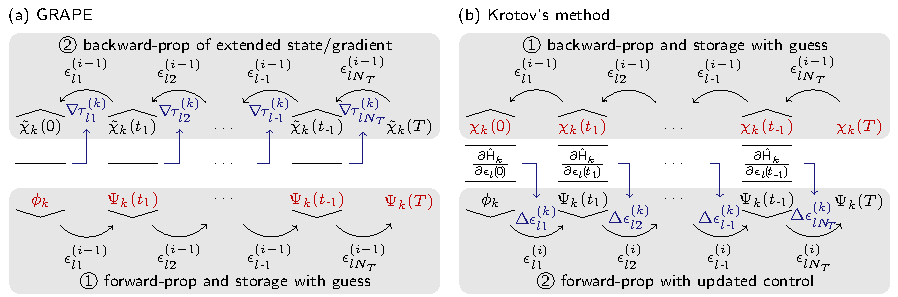
\includegraphics{images/schemes_comparison}
    \end{center}
  \end{textblock}
  \begin{textblock}{14}(1.0,6.75)
    concurrent update \hfill sequential update
  \end{textblock}
  \begin{textblock}{15.5}(0.25,7.75)
    \hfill \footnotesize{--- Goerz \emph{et al.} Quantum 6, 871 (2022)}
  \end{textblock}
\end{frame}

% TODO: comparison

\begin{frame}{QuantumControl.jl}
  \begin{textblock}{15.5}(0.25,1.00)
    \includegraphics<1>[width=\textwidth]{images/JuliaQuantumControl}
  \end{textblock}
\end{frame}

\begin{frame}{Dynamical Generator}
  \begin{textblock}{15.5}(0.25,1.00)
    \includegraphics<1>[width=\textwidth]{images/generator_glossary}
    \includegraphics<2>[width=\textwidth]{images/generator_glossary_g2}
    \includegraphics<3>[width=\textwidth]{images/generator_glossary_g3}
    \includegraphics<4>[width=\textwidth]{images/generator_glossary}
    \includegraphics<5>[width=\textwidth]{images/generator_glossary_g2}
    \includegraphics<6>[width=\textwidth]{images/generator_glossary}
    \includegraphics<7>[width=\textwidth]{images/generator_glossary_g1}
  \end{textblock}
  \begin{textblock}{15.5}(0.25,4.80)
    \begin{center}
      \includegraphics<5>[width=11.55cm]{images/hamiltonian_call}
    \end{center}
  \end{textblock}
  \begin{textblock}{12}(2.0,0.5)
    \begin{center}
      \begin{block}
        \large
        \url{https://github.com/JuliaQuantumControl/JuliaCon2023-Slides}
      \end{block}
    \end{center}
  \end{textblock}
  \note<1>{%
    So the underlying concept that's pretty central in the QuantumControl package is that of a ``dynamical generator''

    which is the object that describes the dynamics of a state

    so a time-dependent Hamiltonian or Liouvillian

    and mathematically the structure that's most directly supported is \dots
  }
  \note<2>{%
    \dots this equation here,

    where you have a drift term, and then you have control operators that get multiplied with a control amplitude

    And the control amplitude depends on one or more control functions epsilon, which are what we're going to be manipulating directly with optimal control.

    So in many cases, the control amplitude is just directly the control function, and then you get \dots
  }
  \note<3>{%

    this linear control Hamiltonian down here

  }
  \note<4>{%

    But in general you could have an amplitude where you add noise on top of your control function, or you have some amplitude that depends non-linearly on one or more controls, like a spin-orbit coupling that's quadratic in the field, or you have some transfer function of a waveform generator, or so many other things.

    So it's really quite flexible.
  }
  \note<5>{%
    And the call to ``hamiltonian'' gives you exactly this structure, where you give tuples of control operators and control amplitudes
  }
  \note<6>{%
    But you could in fact be even more general\dots
  }
  \note<7>{%
    \dots and have operators that depend in some completely arbitrary way on any number of control functions
  }
\end{frame}


\begin{frame}{Generator Interface}
  \begin{textblock}{15.5}(0.25,1.00)
    \includegraphics<1>[width=\textwidth]{images/generator_interface}
    \includegraphics<2>[width=\textwidth]{images/generator_interface_get_controls}
    \includegraphics<3>[width=\textwidth]{images/generator_interface_evaluate}
  \end{textblock}
  \note<1>{%
    So ultimately we just have an abstract interface for what you can use as a dynamical generator

    So you have to be able to \dots
  }
  \note<2>{%
    \dots extract ``controls'', which are scalar functions or arrays, because otherwise you don't have anything to do optimal control on

    And you have to be able to \dots
  }
  \note<3>{%
    \dots evaluate your generator by plugging in values for the controls at a particular point in time

    and that has to give you an ``operator''

    which has its own abstract interface

    but that's basically just an object for which you have to define all the linear algebra operations that you can multiply it to a state.
  }
\end{frame}



\begin{frame}{Propagator Interface}
  \begin{textblock}{15.5}(0.25,1.00)
    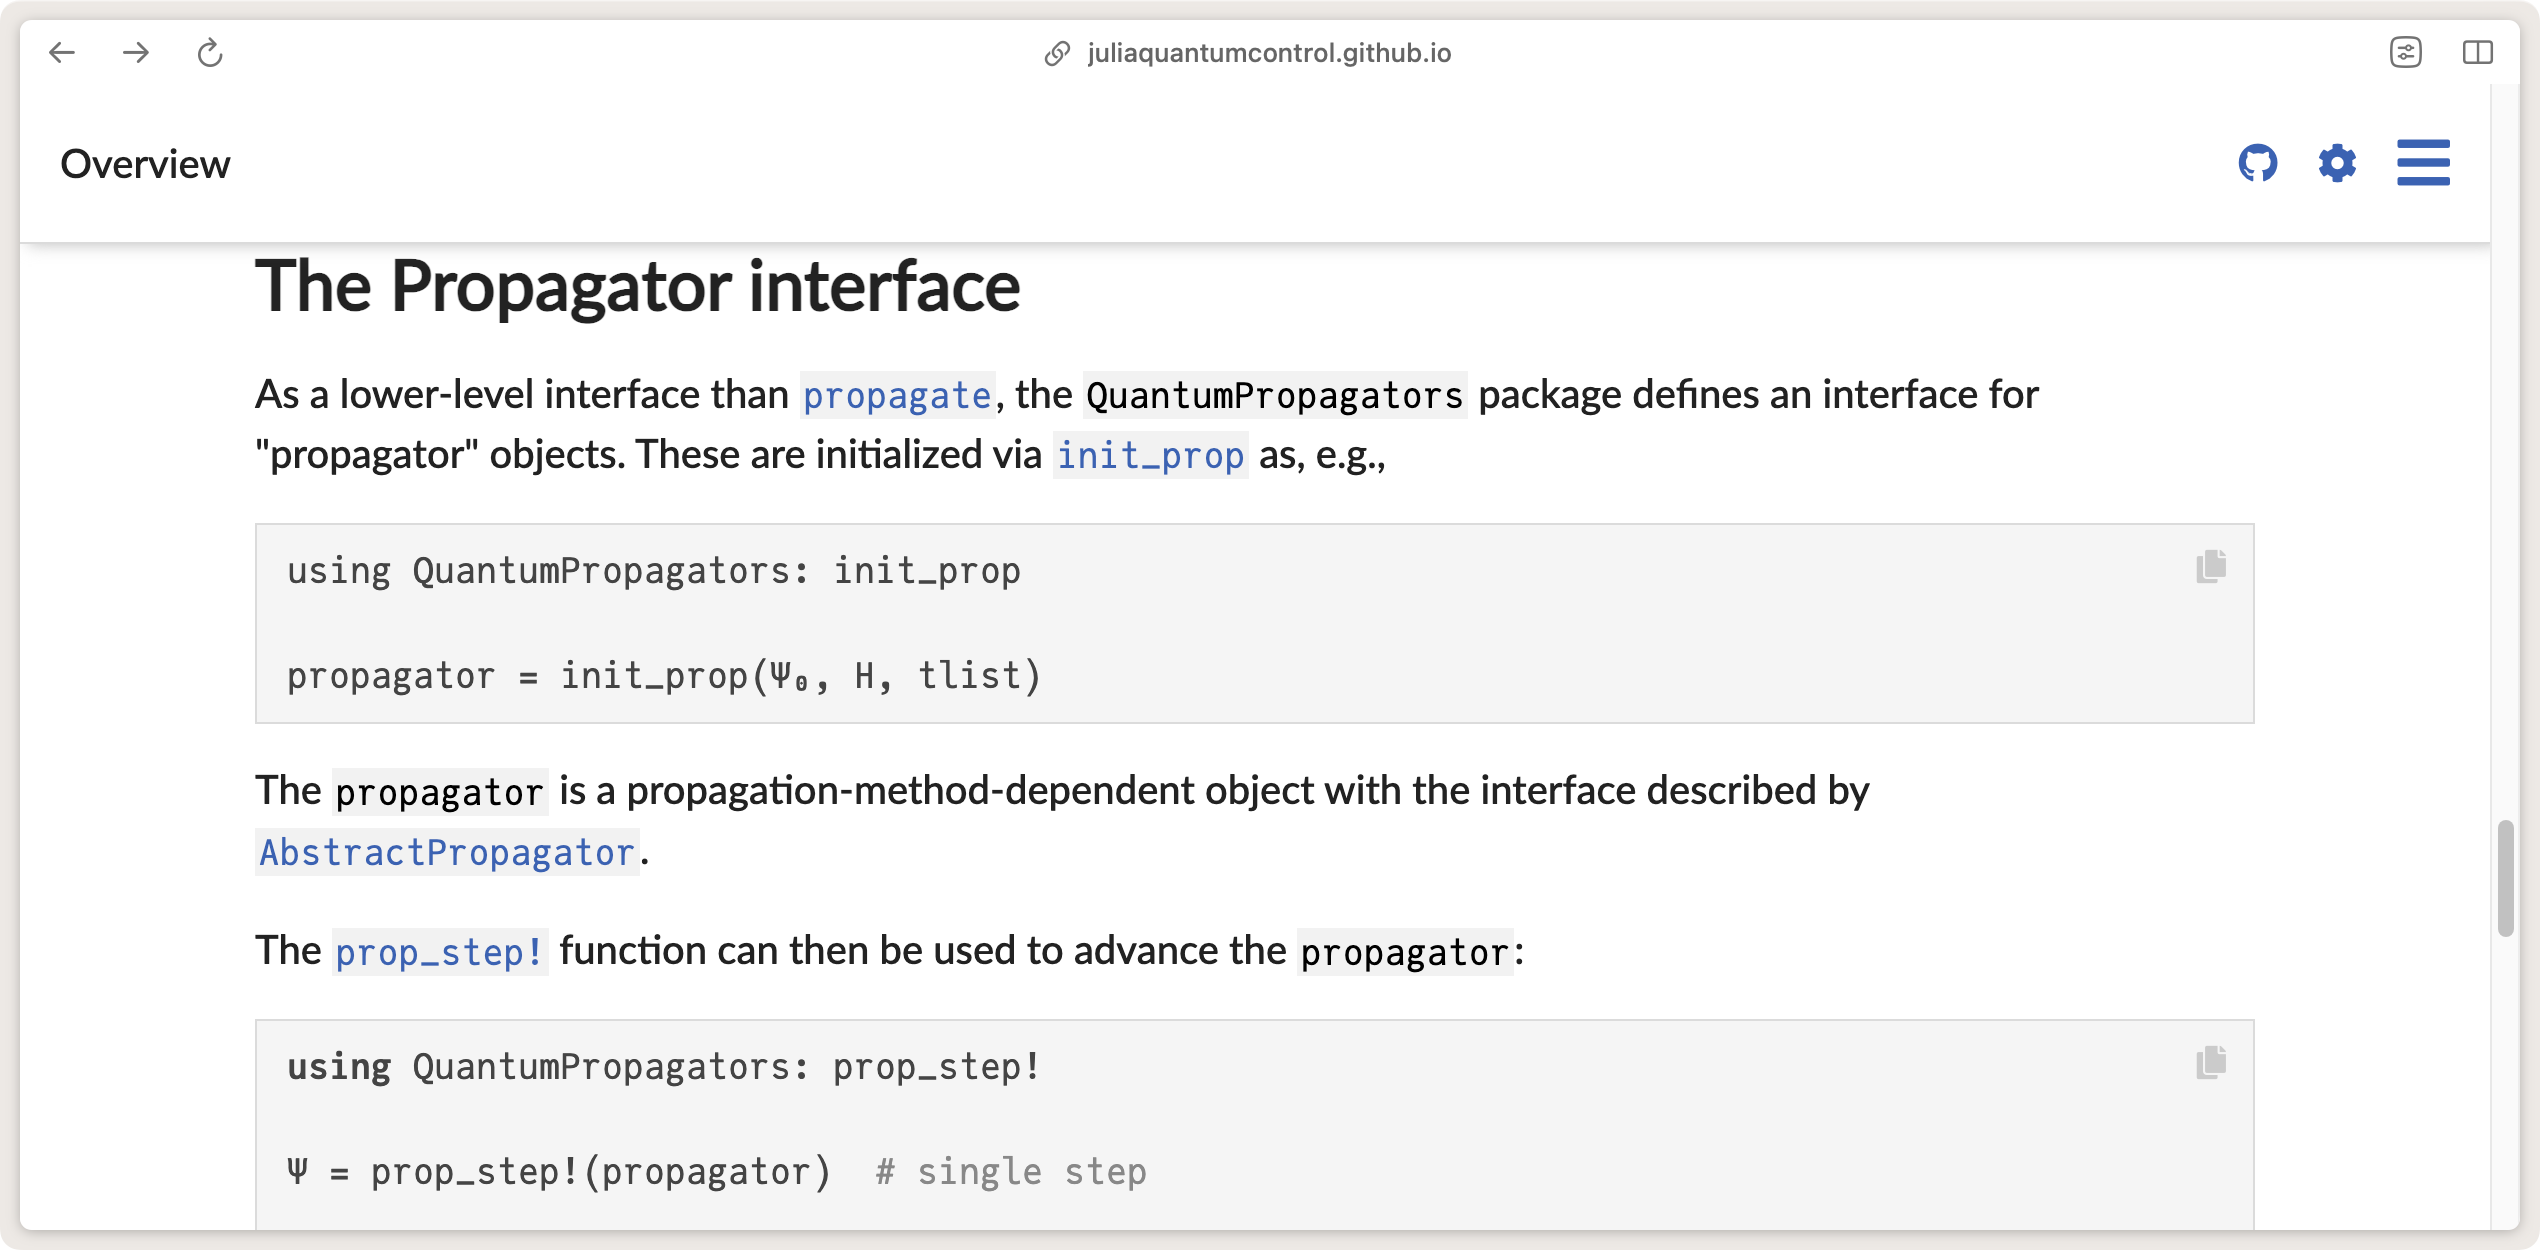
\includegraphics[width=\textwidth]{images/propagator_interface}
  \end{textblock}
  \note<1>{%
    And again this is all implemented via an abstract interface.

    So you can implement propagators where you just need an init-prop function

    And then you can step through the time grid with a prop-step function

    So the Schrödinger equation is implicit in this propagator, but you have have something different like a Gross-Pitaevskii equation, you could define your own propagator according to that interface.
  }
\end{frame}


\begin{frame}{Parametrized Control Fields}
  \begin{textblock}{6.5}(0.5,1.25)
    \includegraphics<1->{images/pulse_examples_continuous}
  \end{textblock}
  \begin{textblock}{7}(7.75,1.35)
    \onslide<2->{%
      \begin{center}
        piecewise-constant pulses
        \par
        $\Rightarrow$ parametrized continuous controls
        \begin{equation*}
          \epsilon(t) = \epsilon(\{u_n\}, t)
        \end{equation*}
      \end{center}
    }
  \end{textblock}
  \begin{textblock}{14}(1.0,5.25)
    \onslide<3->{%
      E.g. CRAB -- Chopped Random (spectral) Basis
      \begin{equation*}
        \epsilon(t)
          = \sum_{i=1}^{10} \left(
              {\color{DarkRed} a_n} \cos(\omega_n t)
              + {\color{DarkRed} b_n} \sin(\omega_n t)
            \right)
      \end{equation*}
      {\footnotesize
        \hfill --- Caneva \textit{et al.} Phys. Rev. A 84, 022326 (2011)
      }
    }
  \end{textblock}
\end{frame}


\begin{frame}{Gradient-free optimization}
  \begin{center}
  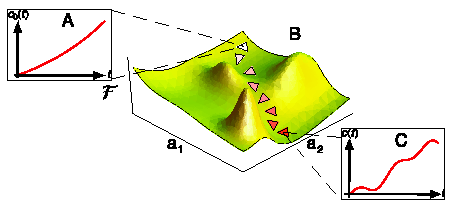
\includegraphics{images/nelder_mead}\\
      {\footnotesize\vspace{-2mm}\hspace{-15mm} Doria et al. PRL 106, 190501 (2011)}
  \end{center}
  \vspace{12pt}
  e.g. Nelder-Mead (simplex), genetic algorithms\dots
\end{frame}

\begin{frame}{Gradients of parametrized pulses}
    \begin{equation*}%
      \begin{pmatrix}
        \frac{\partial \Op{U}}{\partial u_1} \ket{\Psi_k} \\
          \vdots\\
          \frac{\partial \Op{U}}{\partial u_N} \ket{\Psi_k} \\
          \Op{U} \ket{\Psi_k}
        \end{pmatrix}
      = \exp \left[-\ii \TimeOrder \int_0^T \begin{pmatrix}
        \Op{H}(t) & 0 & \dots & 0 &\Op{H}^{(1)}(t) \\
        0 & \Op{H}(t) & \dots & 0 & \Op{H}^{(2)}(t) \\
        \vdots & & \ddots & & \vdots \\
        0 & 0 & \dots & \Op{H}(t) & \Op{H}^{(N)}(t) \\
        0 & 0 & \dots & 0 & \Op{H}(t)
      \end{pmatrix} dt\right]
      \begin{pmatrix} 0 \\ \vdots \\ 0 \\ \ket{\Psi_k} \end{pmatrix}
    \end{equation*}
    \par
    \vspace{5mm}
    \hspace{1cm}
    with $\Op{H}^{(n)}(t) = \frac{\partial \Op{H}(t)}{\partial u_n}$
    \par
    \vspace{5mm}
    {\footnotesize
      \hfill --- ``GOAT'': Machnes \textit{et al.}  Phys. Rev. Lett. 120, 150401 (2018)
    }

\end{frame}

\appendix
\backupbegin

\begin{frame}
\end{frame}

\begin{frame}{Open Quantum Systems}
  \subhead{Lindblad equation:}
  \begin{align*}
  \frac{d}{dt}\Op{\rho}(t)
      & =-i\left[\Op{H},\Op{\rho}(t)\right]+\mathcal{L}_{D}(\Op{\rho}(t))\\
      & =-i\left[\Op{H},\Op{\rho}(t)\right]+\sum_{k}\left(\Op{A}_{k}\Op{\rho}\Op{A}_{k}^{\dagger}-\frac{1}{2}\Op{A}_{k}^{\dagger}\Op{A}_{k}\Op{\rho}-\frac{1}{2}\Op{\rho}\Op{A}_{k}^{\dagger}\Op{A}_{k}\right)
  \end{align*}
  \subhead{Vectorization rule:}
  \begin{equation*}
    \vectorize\left(\Op{A} \Op{\rho} \Op{B} \right)
    = \left(\mat{B}^{T} \otimes \mat{A}\right) \vec{\rho}
  \end{equation*}
  \subhead{Matrix representation of Lindbladian:}
  \begin{equation*}
    \mat{L} =
      -i (\identity \otimes \mat{H}) + i (\mat{H}^T \otimes \identity)
      + \sum_k \left[
        (\mat{A}_k^\dagger)^T \otimes \mat{A}_k
        - \half \left(\identity \otimes \mat{A}_k^\dagger \mat{A}_k\right)
        - \half \left((\mat{A}_k^\dagger \mat{A}_k)^T \otimes \identity\right)
        \right]\
  \end{equation*}
  \hfill {\footnotesize --- Goerz \textit{et. al.} arXiv:1312.0111v2 (2021), Appendix B}
\end{frame}

\backupend

\end{document}
